\subsection{测度的逆系统}

定义 1. --- 设 \(\mathcal{T} = (\mathrm{T}_i, p_{ij})\) 是以 I 为指标的拓扑空间逆系统。称测度的逆系统（分别地，测度的子逆系统）

为 \(\mathcal{T}\) 上的一个族 \((\mu_i)_{i\in I}\)，其中 \(\mu_i\) 是 \(\mathrm{T}_i\) 上的有界测度，对所有 \(i\in \mathrm{I}\) 均如此，并且 \(\mu_i = p_{ij}(\mu_j)\)（分别地，\(\mu_i\geqslant p_{ij}(\mu_j)\)）对 \(i\leqslant j\) 成立。

命题 3. --- 设给定以 I 为指标的拓扑空间逆系统 \(\mathcal{T} = (\mathrm{T}_i, p_{ij})\)、拓扑空间 T、相容且分离的连续映射族 \(p_i: \mathrm{T} \to \mathrm{T}_i\)（\(i \in \mathrm{I}\)）以及测度子逆系统 \((\mu_i)_{i \in \mathrm{I}}\)（它是在 \(\mathcal{T}\) 上的）。对 T 的每个紧子集 K，置

\[
\mathrm{J} (\mathrm{K}) = \inf _ {i \in \mathrm{I}} \mu_ {i} ^ {\bullet} (p _ {i} (\mathrm{K})).\tag{1}
\]

则 T 上存在且仅存在一个有界测度 \(\pi\)，使得对 T 的每个紧子集 K 都有 \(\pi^{\bullet}(\mathrm{K}) = \mathrm{J}(\mathrm{K})\)。有 \(\mu_i \geqslant p_i(\pi)\) 对所有 \(i \in I\) 成立，并且 \(\pi\) 是满足此条件的 T 上最大测度。

先证明 \(\mathrm{J}(\mathrm{K})\) 是 \(\mu_i^\bullet (p_i(\mathrm{K}))\) 关于有向预序集 I 的截段滤子 \(\mathfrak{F}\) 的极限：为此，只须（GT, IV, §5, No.~2, Th. 2）证明 \(\mu_i^\bullet (p_i(\mathrm{K})) \geqslant \mu_j^\bullet (p_j(\mathrm{K}))\) 对 \(i \leqslant j\) 成立；现在置 \(\mu_{ij}' = p_{ij}(\mu_j)\)，则有 \(\mu_{ij}' \leqslant \mu_i\) 以及 \(p_j(\mathrm{K}) \subset \overline{p}_{ij}^{-1}(p_i(\mathrm{K}))\)，从而

\[
\mu_ {j} ^ {\bullet} \big (p _ {j} (\mathrm{K}) \big) \leqslant \mu_ {j} ^ {\bullet} \big (\overline{p}_{ij}^{-1} (p _ {i} (\mathrm{K})) \big) = (\mu_ {i j} ^ {\prime}) ^ {\bullet} \big (p _ {i} (\mathrm{K}) \big) \leqslant \mu_ {i} ^ {\bullet} \big (p _ {i} (\mathrm{K}) \big).
\]

现在来研究函数 J 的性质：

\begin{enumerate}
\def\labelenumi{\arabic{enumi})}
\item
  显然，\(\mathrm{J}(\mathbf{K})\leqslant \mathrm{J}(\mathbf{L})\) 当 \(\mathbf{K}\subset \mathbf{L}\) 时成立。
\item
  设 \(\mathbf{K}\) 和 \(\mathbf{L}\) 是 \(\mathbf{T}\) 的两个紧子集。对每个 \(i \in \mathbf{I}\)，有 \(p_i(\mathbf{K} \cup \mathbf{L}) = p_i(\mathbf{K}) \cup p_i(\mathbf{L})\)，从而
\end{enumerate}

\[
\mu_ {i} ^ {\bullet} \left(p _ {i} (\mathrm{K} \cup \mathrm{L})\right) \leqslant \mu_ {i} ^ {\bullet} \left(p _ {i} (\mathrm{K})\right) + \mu_ {i} ^ {\bullet} \left(p _ {i} (\mathrm{L})\right);
\]

关于滤子 \(\mathfrak{F}\) 取极限，得到 \(\mathrm{J}(\mathrm{K} \cup \mathrm{L}) \leqslant \mathrm{J}(\mathrm{K}) + \mathrm{J}(\mathrm{L})\)。

\begin{enumerate}
\def\labelenumi{\arabic{enumi})}
\setcounter{enumi}{2}
\tightlist
\item
  假设紧集 K 和 L 不相交。由第 1 号命题 2，存在 \(i \in I\)，使得 \(p_j(K) \cap p_j(L) = \varnothing\) 对 \(j \geqslant i\) 成立。因此对 \(j \geqslant i\) 有
\end{enumerate}

\[
\mu_ {j} ^ {\bullet} \left(p _ {j} (\mathrm{K} \cup \mathrm{L})\right) = \mu_ {j} ^ {\bullet} \left(p _ {j} (\mathrm{K})\right) + \mu_ {j} ^ {\bullet} \left(p _ {j} (\mathrm{L})\right),
\]

从而关于滤子 F 取极限得到 \(\mathrm{J}(\mathrm{K}\cup\mathrm{L})=\mathrm{J}(\mathrm{K})+\mathrm{J}(\mathrm{L})\)。

\begin{enumerate}
\def\labelenumi{\arabic{enumi})}
\setcounter{enumi}{3}
\tightlist
\item
  设 \((\mathbf{K}_{\alpha})_{\alpha \in \mathbf{A}}\) 是 T 的紧子集的一个递减有向族，其交为 K。由第 1 节第 1 号命题，\(p_i(\mathbf{K}) = \bigcap_{\alpha \in \mathbf{A}} p_i(\mathbf{K}_{\alpha})\)，并且
\end{enumerate}

因此 \(\mu_i^\bullet (p_i(\mathbf{K})) = \inf_{\alpha \in \mathbf{A}}\mu_i^\bullet (p_i(\mathbf{K}_\alpha))\) 对所有 \(i\in I\) 成立（§1, No.~6, Prop. 5 的推论）。由此推出

\[
\begin{array}{r l} \mathrm{J(K)} & = \inf _ {i \in \mathrm{I}} \mu_ {i} ^ {\bullet} (p _ {i} (\mathrm{K})) = \inf _ {i \in \mathrm{I}} \inf _ {\alpha \in \mathrm{A}} \mu_ {i} ^ {\bullet} (p _ {i} (\mathrm{K} _ {\alpha})) \\ & = \inf _ {\alpha \in \mathrm{A}} \inf _ {i \in \mathrm{I}} \mu_ {i} ^ {\bullet} (p _ {i} (\mathrm{K} _ {\alpha})) = \inf _ {\alpha \in \mathrm{A}} \mathrm{J(K} _ {\alpha}). \end{array}
\]

\begin{enumerate}
\def\labelenumi{\arabic{enumi})}
\setcounter{enumi}{4}
\tightlist
\item
  取定 \(i \in I\)，置 \(c = \mu_i^\bullet(T_i)\)。则 \(c\) 有限且 \(J(K) \leqslant \mu_i^\bullet(p_i(K)) \leqslant \mu_i^\bullet(T_i)\)，故有 \(J(K) \leqslant c\)，对每个紧集 \(K\)（\(T\) 中）成立。前述性质允许应用 §3 第 1 号定理；于是存在且仅存在一个有界测度 \(\pi\) 定义在 \(T\) 上，使 \(\pi^\bullet(K) = J(K)\) 对每个紧子集 \(K\)（\(T\) 中）成立。对每个 \(i \in I\)，记 \(\nu_i\) 为 \(T_i\) 上的测度，它是 \(\pi\) 在 \(p_i\) 下的像。取 \(i \in I\)、\(A\) 为 \(T_i\) 的紧子集，并令 \(\mathfrak{L}\) 为 \(\overline{p}_i^1(A)\) 的紧子集所成的集合。由 §1 第 2 号备注 3，有 \(\pi^\bullet(\overline{p}_i^1(A)) = \sup_{K \in \mathfrak{L}} \pi^\bullet(K)\)；此外，\(\nu_i^\bullet(A) = \pi^\bullet(\overline{p}_i^1(A))\)，且有 \(J(K) = \pi^\bullet(K)\) 对 \(K \in \mathfrak{L}\) 成立，从而 \(\nu_i^\bullet(A) = \sup_{K \in \mathfrak{L}} J(K)\)。对 \(K \in \mathfrak{L}\)，有 \(p_i(K) \subset A\)，从而 \(J(K) \leqslant \mu_i^\bullet(p_i(K)) \leqslant \mu_i^\bullet(A)\)，最后得到 \(\nu_i^\bullet(A) \leqslant \mu_i^\bullet(A)\)。由于 \(A\) 是 \(T_i\) 中任意的紧集，故 \(\nu_i \leqslant \mu_i\)。命题的最后一个断言显然成立。
\end{enumerate}

证毕。

定理 1（Prokhorov）。 --- 设 \(\mathcal{T} = (\mathrm{T}_{i}, p_{ij})\) 是以 I 为指标的拓扑空间逆系统，T 是拓扑空间，\((p_{i})_{i \in I}\) 是相容且分离的连续映射族 \(p_{i}: \mathrm{T} \to \mathrm{T}_{i}\)。最后，设 \((\mu_{i})_{i \in I}\) 是 \(\mathcal{T}\) 上的测度逆系统。

为使存在有界测度 \(\mu\) 定义在 \(\mathbf{T}\) 上，满足 \(p_i(\mu) = \mu_i\) 对所有 \(i \in \mathbf{I}\) 成立，以下条件成立是必要且充分的：

\begin{enumerate}
\def\labelenumi{(\Alph{enumi})}
\setcounter{enumi}{15}
\tightlist
\item
  对每个 \(\varepsilon > 0\)，存在紧子集 \(K\)（属于 \(T\)），使得 \(\mu_i^\bullet(T_i - p_i(K)) \leqslant \varepsilon\) 对所有 \(i \in I\) 成立。
\end{enumerate}

若此条件成立，测度 \(\mu\) 唯一确定，并且

\[
\mu^ {\bullet} (\mathbf {K}) = \inf _ {i} \mu_ {i} ^ {\bullet} (p _ {i} (\mathbf {K}))\tag{2}
\]

对每个紧集 \(\mathbf{K}\)（属于 \(\mathbf{T}\)）都成立。

先证明 \(\mu\) 的唯一性。设 \(\mu\) 是 T 上的有界测度，满足 \(p_i(\mu) = \mu_i\) 对所有 \(i \in I\) 成立。设 K 是 T 的紧子集；由第 1 节第 2 号命题，集合 K 是 T 的闭子集递减有向族 \(\left(\overline{p_i^1}(p_i(K))\right)_{i \in I}\) 的交。由 §1 第 6 号命题 5 的推论，因而有

\[
\mu^ {\bullet} (\mathrm{K}) = \inf _ {i \in \mathrm{I}} \mu^ {\bullet} \left(\bar {p} _ {i} ^ {- 1} (p _ {i} (\mathrm{K}))\right) = \inf _ {i \in \mathrm{I}} \mu_ {i} ^ {\bullet} \left(p _ {i} (\mathrm{K})\right),
\]

这就证明了公式 (2)。由于在紧集全体上相同的两个测度相等（§1, No.~2, Prop. 2 的推论），故 \(\mu\) 唯一。

由命题 3，存在有界测度 \(\pi\) 定义在 \(\mathbf{T}\) 上，使得 \(\pi^{\bullet}(\mathbf{K}) = \inf_{i\in I}\mu_i^\bullet (p_i(\mathbf{K}))\) 对每个紧子集 \(\mathbf{K}\)（属于 \(\mathbf{T}\)）成立。由公式 (2)，存在有界测度 \(\mu\) 定义在 \(\mathbf{T}\) 上，满足 \(p_i(\mu) = \mu_i\) 对所有 \(i\in I\) 成立，因而等价于关系：

\[
\left(\mathrm{P} ^ {\prime}\right) p _ {i} (\pi) = \mu_ {i} \text { for all } i \in \mathrm{I}.
\]

当 \(i \leqslant j\) 时，有 \(\mu_i = p_{ij}(\mu_j)\)，从而 \(\mu_i^\bullet (\mathbf{T}_i) = \mu_j^\bullet (\mathbf{T}_j)\)；由于 I 是有向的，存在有限数 \(c \geqslant 0\)，使得 \(\mu_i^\bullet (\mathbf{T}_i) = c\) 对所有 \(i \in I\) 成立。由命题 3，测度 \(\mu_i - p_i(\pi)\) 为正，因此它为零当且仅当其总质量为零，即 \(\mu_i(\mathbf{T}_i) = p_i(\pi)^\bullet (\mathbf{T}_i)\)。由于 \(p_i(\pi)^\bullet (\mathbf{T}_i) = \pi^\bullet (\mathbf{T})\)，条件 \((\mathbf{P}')\) 遂等价于 \(\pi^\bullet (\mathbf{T}) = c\)，即（§1, No.~2, 备注 3）等价于性质：

\((\mathbf{P}^{\prime \prime})\sup_{K\in \mathfrak{K}}\pi^{\bullet}(\mathbf{K}) = c\)，其中 \(\mathfrak{K}\) 是 T 的紧子集所成的集合。

现在，对于 \(\mathbf{K} \in \mathfrak{K}\) ，有

\[
\pi^ {\bullet} (\mathrm{K}) = \inf _ {i \in \mathrm{I}} \mu_ {i} ^ {\bullet} (p _ {i} (\mathrm{K})) = c - \sup _ {i \in \mathrm{I}} \mu_ {i} ^ {\bullet} (\mathrm{T} _ {i} - p _ {i} (\mathrm{K}))
\]

而此公式立即推出 (P) 与 \((\mathbf{P}^{\prime \prime})\) 等价。

Q.E.D.

设 \((\mathrm{T}_{i}, p_{ij})\) 是拓扑空间的逆系统。置 \(\mathrm{T} = \varprojlim \mathrm{T}_{i}\)，并记 \(p_{i}\) 为从 \(\mathrm{T}\) 到 \(\mathrm{T}_{i}\) 的典范映射。推广第 III 章 §4 第 5 号定义 2，称 \(\mu\) 为定义在 \(\mathrm{T}\) 上的有界测度，是测度逆系统 \((\mu_{i})_{i \in \mathrm{I}}\) 的逆极限，如果 \(\mu_{i} = p_{i}(\mu)\) 对所有 \(i \in \mathrm{I}\) 成立。定理 1 给出了逆极限测度存在的判据。当空间 \(\mathrm{T}_{i}\) 紧且映射 \(p_{ij}\) 为满射时，\(\mathrm{T}\) 紧，并且 \(p_{i}(\mathrm{T}) = \mathrm{T}_{i}\) 对每个 \(i \in \mathrm{I}\) 成立；因此条件 (P) 得到满足，此时我们得到第 III 章 §4 第 5 号命题 8(iv)。

备注。 --- 设 \((\mu_{i})_{i\in\mathbb{I}}\) 是空间逆系统 \(\mathcal{T}=(\mathrm{T}_{i},p_{ij})\) 上的测度逆系统。设给定拓扑空间 \(T'\) 及连续映射 \(p_{i}^{\prime}:T^{\prime}\to T_{i}\)；假设族 \((p_{i}^{\prime})_{i\in\mathbb{I}}\) 相容，但不一定分离。如果族 \((p_{i}^{\prime})_{i\in\mathbb{I}}\) 满足 Prokhorov 条件 (P)，则存在测度 \(\mu^{\prime}\)（不一定唯一），定义在 \(T^{\prime}\) 上，使得 \(p_{i}^{\prime}(\mu^{\prime})=\mu_{i}\) 对所有 \(i\in I\) 成立。

为此，置 \(\mathbf{T} = \varprojlim \mathbf{T}_i\) 和 \(p' = (p_i')_{i\in I}\)，并记 \(p_i\) 为从 \(\mathbf{T}\) 到 \(\mathbf{T}_i\) 的典范映射；Prokhorov 条件由 \(\mathbf{T}\) 与 \(p_i\) 满足，因为 \(p_i(p'(K')) = p'_i(K')\)，且 \(p'(K')\) 在 \(\mathbf{T}\) 中紧，对 \(\mathbf{K}'\) 的每个紧子集 \(\mathbf{T}'\) 都如此。由定理 1，存在有界测度 \(\mu\) 定义在 \(\mathbf{T}\) 上，满足 \(p_i(\mu) = \mu_i\) 对所有 \(i\in I\) 成立。设 \(\mathbf{K}'\) 是 \(\mathbf{T}'\) 中的紧集；则 \(\mu^\bullet (p'(K')) = \inf_{i\in I}\mu_i^\bullet (p_i'(K'))\)，

从而

\[
\mu^ {\bullet} \left(\mathrm{T} - p ^ {\prime} \left(\mathrm{K} ^ {\prime}\right)\right) = \sup _ {i \in \mathrm{I}} \mu_ {i} ^ {\bullet} \left(\mathrm{T} _ {i} - p _ {i} ^ {\prime} \left(\mathrm{K} ^ {\prime}\right)\right).
\]

令 \(\varepsilon > 0\)；由于 Prokhorov 条件 (P) 由 \(p_i'\) 满足，所以可以找到紧子集 \(K'\)（属于 \(T'\)），使得 \(\mu^\bullet(T - p'(K')) \leqslant \varepsilon\)。于是 §2 第 4 号命题 8 说明存在有界测度 \(\mu'\)，定义在 \(T'\) 上，满足 \(\mu = p'(\mu')\)，从而 \(\mu_i = p_i(\mu) = p_i(p'(\mu')) = p_i'(\mu')\) 对所有 \(i \in I\) 成立。

\subsection{可数逆系统的情形}

定理 2. --- 假设有向预序集 I 有一个可数共尾子集。设 \(\mathcal{T} = (\mathrm{T}_i, p_{ij})\) 是拓扑空间的逆系统，\(\mathrm{T} = \varprojlim \mathrm{T}_i\)，且 \(p_i\) 是从 \(\mathrm{T}\) 到 \(\mathrm{T}_i\) 的典范映射。则 \((\mu_i)_{i \in \mathrm{I}}\) 上的每个测度逆系统 \(\mathcal{T}\) 都有逆极限。

先处理 I = N 的情形，置 \(q_{n} = p_{n,n+1}\)。令 \(\varepsilon > 0\)。递归定义紧集序列 \(L_{n} \subset T_{n}\) 如下：\(L_{0}\) 是 \(T_{0}\) 的紧子集，满足 \(\mu_{0}^{\bullet}(T_{0} - L_{0}) \leqslant \varepsilon / 2\)；并且对 \(n \geqslant 0\)，紧集 \(L_{n+1}\) 包含于 \(\overline{q}_{n}^{-1}(L_{n})\) 中并满足

\[
\mu_ {n + 1} ^ {\bullet} \big (\overline{q}_{n}^{-1} (\mathrm{L} _ {n}) - \mathrm{L} _ {n + 1} \big) \leqslant \varepsilon / 2 ^ {n + 2}.
\]

根据 §1 第 2 号备注 3，这一构造是可能的。我们有

\[
\begin{array}{r l} & {\mu_ {n + 1} ^ {\bullet} (\mathrm{T} _ {n + 1} - \mathrm{L} _ {n + 1}) = \mu_ {n + 1} ^ {\bullet} \big (\mathrm{T} _ {n + 1} - \overline{q}_{n}^{-1} (\mathrm{L} _ {n}) \big) + \mu_ {n + 1} ^ {\bullet} \big (\overline{q}_{n}^{-1} (\mathrm{L} _ {n}) - \mathrm{L} _ {n + 1} \big)} \\ & {\qquad \leqslant \mu_ {n + 1} ^ {\bullet} \big (\mathrm{T} _ {n + 1} - \overline{q}_{n}^{-1} (\mathrm{L} _ {n}) \big) + \varepsilon / 2 ^ {n + 2}} \\ & {\qquad = \mu_ {n} ^ {\bullet} (\mathrm{T} _ {n} - \mathrm{L} _ {n}) + \varepsilon / 2 ^ {n + 2}} \end{array}
\]

因为 \(\mu_{n} = q_{n}(\mu_{n + 1})\)；对 \(p\) 作归纳，得到

\[
\mu_ {p} ^ {\bullet} \left(\mathrm{T} _ {p} - \mathrm{L} _ {p}\right) \leqslant \varepsilon \left(1 - 1 / 2 ^ {p + 1}\right) \leqslant \varepsilon .
\]

由于 \(\mathbf{T}\) 是 \(\prod_{n\in \mathbf{N}}\mathrm{T}_n\) 的闭子空间，而积空间 \(\prod_{n\in \mathbf{N}}\mathrm{L}_n\) 是紧的，所以 \(\mathbf{L} = \mathbf{T}\cap \prod_{n\in \mathbf{N}}\mathrm{L}_n = \bigcap_{n\in \mathbf{N}}\overline{p}_n^1 (\mathrm{L}_n)\) 是 \(\mathbf{T}\) 的紧子集。取 \(n\in \mathbf{N}\)；有 \(p_n(\mathrm{L}) = \bigcap_{m\geqslant n}p_{nm}(\mathrm{L}_m)\)（GT, I, §9, No.~6, 命题 8），且 \(p_{nm}(\mathrm{L}_m)\supset p_{nm'}(\mathrm{L}_{m'})\) 对 \(m^{\prime}\geqslant m\geqslant n\) 成立，从而

\[
\mu_ {n} ^ {\bullet} \big (\mathrm{T} _ {n} - p _ {n} (\mathrm{L}) \big) = \lim _ {m \rightarrow \infty} \mu_ {n} ^ {\bullet} \big (\mathrm{T} _ {n} - p _ {n m} (\mathrm{L} _ {m}) \big).
\]

但是，对 \(m \geqslant n\)，测度 \(\mu_{n}\) 是 \(\mu_{m}\) 在 \(p_{nm}\) 下的像，从而

\[
\mu_ {n} ^ {\bullet} \left(\mathrm{T} _ {n} - p _ {n m} (\mathrm{L} _ {m})\right) = \mu_ {m} ^ {\bullet} \left(\mathrm{T} _ {m} - \bar {p} _ {n m} ^ {- 1} (p _ {n m} (\mathrm{L} _ {m}))\right) \leqslant \mu_ {m} ^ {\bullet} \left(\mathrm{T} _ {m} - \mathrm{L} _ {m}\right) \leqslant \varepsilon ;
\]

关于 \(m\) 取极限，得到 \(\mu_n^\bullet (\mathrm{T}_n - p_n(\mathrm{L})) \leqslant \varepsilon\)。换言之，Prokhorov 条件 (P) 得到满足，并且 T 上存在有界测度 \(\mu\)，使得 \(\mu_n = p_n(\mu)\) 对所有 \(n \in \mathbf{N}\) 成立（第 2 号定理 1）。

现在处理一般情形：I 中存在递增的共尾序列 \((i_{n})_{n\in\mathbf{N}}\)。映射 \(t\mapsto\left(p_{i_{n}}(t)\right)_{n\in\mathbf{N}}\) 将 T 同胚映到逆系统 \((\mathrm{T}_{i_{n}},p_{i_{n}i_{m}})\) 的逆极限（GT, I, §4, No.~4）。由证明的第一部分，因而存在有界测度 \(\mu\) 定义在 T 上，使得 \(\mu_{i_{n}}=p_{i_{n}}(\mu)\) 对所有 \(n\in N\) 成立。取 \(i\in I\)；存在 \(n\in N\) 使得 \(i\leqslant i_{n}\)，从而

\[
p _ {i} (\mu) = p _ {i i _ {n}} \left(p _ {i _ {n}} (\mu)\right) = p _ {i i _ {n}} \left(\mu_ {i _ {n}}\right) = \mu_ {i}.\tag{Q.E.D.}
\]

定理 2 常用于如下情形：设 D 是可数集，\((\mathrm{X}_{t})_{t\in\mathrm{D}}\) 是拓扑空间族。令 F 为 D 的有限子集按包含关系构成的集合。对于 F 中的 J，置 \(X_{J}=\prod_{t\in J}X_{t}\)，而对 \(J\subset J'\)，令 \(p_{JJ'}\) 为从 \(X_{J'}\) 到部分积 \(X_{J}\) 的典范投影。再置 \(X=\prod_{t\in D}X_{t}\)，并记 \(p_{J}\) 为从 X 到部分积 \(X_{J}\) 的典范投影。容易证明（参见 S, III, §7, No.~2, 备注 3），族 \((p_{J})_{J\in\mathfrak{F}}\) 将 X 同胚映到 \(\varprojlim X_{J}\)。于是，测度逆系统就是定义在 \(\mu_{J}\) 上的有界测度族 \(X_{J}\)，满足 \(\mu_{J}=p_{JJ'}(\mu_{J'})\) 对 \(J\subset J'\) 成立。存在且仅存在一个定义在 X 上的有界测度 \(\mu\)，使得 \(\mu_{J}=p_{J}(\mu)\) 对 D 的每个有限子集 J 都成立（Kolmogoroff 定理）。有时称 \(\mu\) 为 \(\prod_{t\in D}X_{t}\) 上具有边缘测度 \(\mu_{J}\) 的测度。

特别地，设对每个 \(t \in D\)，给定定义在 \(\nu_{t}\) 上且总质量为 1 的测度 \(X_{t}\)。对 D 的每个有限子集 J，置 \(\mu_{J} = \bigotimes_{t \in J} \nu_{t}\)。设 \(J \subset J'\) 是 D 的两个有限子集，并令 \(K = J' - J\)；将 \(X_{J'}\) 与 \(X_{J} \times X_{K}\) 视同，有 \(\mu_{J'} = \mu_{J} \otimes \mu_{K}\)，而由于测度 \(\mu_{K}\) 的总质量为 1，\(\mu_{J} \otimes \mu_{K}\) 在 \(X_{J}\) 上的投影等于 \(\mu_{J}\)。具有边缘测度 \(\mu_{J}\) 的 X 上测度记为 \(\bigotimes_{t \in D} \nu_{t}\)，称为族 \((\nu_{t})_{t \in D}\) 的积。当空间 \(X_{t}\) 紧时，我们得到第 III 章 §4 第 6 号的构造。

\section{完全正则空间上的测度}

若 \(\mathbf{T}\) 是拓扑空间，且 \(\overline{\mathbf{F}}\) 是 Banach 空间，则记号 \(\mathcal{C}^b (\mathrm{T};\mathbf{F})\) 表示定义在 \(\mathbf{T}\) 上、取值于 \(\mathbf{F}\) 的有界连续函数空间，并赋予一致收敛范数。当 \(\mathbf{F} = \mathbf{R}\) 时，此记号简写为 \(\mathcal{C}^b (\mathrm{T})\)；若无歧义，也简写为 \(\mathcal{C}^b\)，并以 \(\mathcal{C}_+^b (\mathrm{T})\) 或 \(\mathcal{C}_+^b\) 表示 \(\mathcal{C}^b (\mathrm{T})\) 中正函数所成的锥。\(\mathbf{T}\) 上有界复测度空间记为 \(\mathcal{M}^b (\mathrm{T};\mathbf{C})\)，有界实测度空间记为 \(\mathcal{M}^b (\mathrm{T})\) 或 \(\mathcal{M}^b\)，有界正测度所成的锥记为 \(\mathcal{M}_+^b (\mathrm{T})\) 或 \(\mathcal{M}_+^b\)。

\subsection{测度与有界连续函数}

回忆（GT, IX, §1, No.~5, 定义 4），拓扑空间 T 称为完全正则的，是指它可一致化且为豪斯多夫空间。这等价于（同上，命题 3）T 同胚于某个紧空间的子空间。若 T 完全正则，则 T 上每个正的下半连续函数 f 都是由满足 \(\mathcal{C}_{+}^{b}(T)\) 的 \(\leqslant f\) 元素构成的递增有向集的上包络；每个正的有界上半连续函数 g 都是由满足 \(\mathcal{C}_{+}^{b}(T)\) 的 \(\geqslant g\) 元素构成的递减有向集的下包络（同上，§1, No.~6, 命题 5）。我们将需要以下引理：

引理。 --- 设 T 是完全正则空间，K 是 T 的紧子集，U 是包含 K 的 T 的开子集。

\begin{enumerate}
\def\labelenumi{\alph{enumi})}
\item
  存在开子集 \(\mathbf{U}'\)（属于 \(\mathbf{T}\)），使得 \(\mathbf{K} \subset \mathbf{U}' \subset \overline{\mathbf{U}'} \subset \mathbf{U}\)。
\item
  设 \(f\) 是定义在 \(K\) 上、取值于区间 \(I\)（属于 \(\mathbf{R}\)）（分别地，取值于 \(\mathbf{C}\)）的连续函数。存在定义在 \(f'\) 上、取值于 \(T\)（分别地，取值于 \(I\)）的有界连续函数 \(\mathbf{C}\)，它延拓 \(f\) 且在 \(T - U\) 上为零。
\end{enumerate}

只须处理 T 是紧空间 X 的子空间的情形。设 V 是 X 的开子集，满足 \(V \cap T = U\)；记 \(V'\) 为 X 中包含 K 且满足 \(\overline{V'} \subset V\) 的开集，记 g 为 X 上取值于 I（分别地，取值于 C）、延拓 f 且在 X - V 上为零的连续函数（GT, IX, §4, No.~1, 命题 1）。取 \(U' = V' \cap T\) 即满足 a)，取 \(f'\) 为 g 在 T 上的限制即满足 b)。

命题 1. --- 设 T 是完全正则空间。

\begin{enumerate}
\def\labelenumi{\alph{enumi})}
\tightlist
\item
  设 \(\mu\) 是 \(\mathbf{T}\) 上的正测度，\(f\) 是满足 \(\geqslant 0\) 且定义在 \(\mathbf{T}\) 上的数值函数，并且是下半连续的（分别地，是上半连续的、有限的、有紧支集的）。则
\end{enumerate}

\[
\mu^ {\bullet} (f) = \sup _ {g \in I _ {f}} \mu^ {\bullet} (g) \quad (\text { resp. } \mu^ {\bullet} (f) = \inf _ {g \in S _ {f}} \mu (g)),\tag{1}
\]

其中 \(I_{f}\)（分别地，\(S_{f}\)）表示满足 \(0 \leqslant g \leqslant f\)（分别地，\(g \geqslant f\)）的有界连续函数 g 所成的集合。

\begin{enumerate}
\def\labelenumi{\alph{enumi})}
\setcounter{enumi}{1}
\tightlist
\item
  设 \(\theta\) 是 \(\mathbf{T}\) 上的复测度，\(f\) 是满足 \(\geqslant 0\) 且定义在 \(\mathbf{T}\) 上的数值函数，并且是下半连续的。则
\end{enumerate}

\[
| \theta | ^ {\bullet} (f) = \sup _ {g} | \theta (g) |,\tag{2}
\]

其中 \(g\) 遍历有界且对 \(|\theta|\) 可积的连续复函数所成集合，并满足 \(|g| \leqslant f\)。

公式 (1) 中的第一个公式显然成立，因为 \(I_{f}\) 是由连续函数组成的递增有向集，其上包络为 f，可以应用 §1 第 6 号命题 5。如果证明 \(S_{f}\) 含有一个对 \(\mu\) 可积的有界连续函数，同一命题就能推出第二个公式。于是，设 K 是 f 的支集，M 是 f 的上确界；由于 K 紧，M 有限（GT, IV, §6, No.~2, Th. 3）。取包含 K 且满足 \(\mu^{\bullet}(U) < +\infty\) 的开集 U；由（引理）存在取值于 {[}0, M{]}、在 K 上等于 M 且在 U 外为零的连续函数 g；于是 \(g \in S_{f}\)，并且 \(\mu^{\bullet}(g) \leqslant M\mu^{\bullet}(U) < +\infty\)。

转到 \(b\)。显然只须证明 \(|\theta|^{\bullet}(f) \leqslant \sup |\theta(g)|\)。

设 \(a\) 和 \(b\) 是满足 \(a < b < |\theta|^{\bullet}(f)\) 的两个实数。由 (1)，存在函数 \(h \in \mathcal{C}_{+}^{b}(\mathrm{T})\)，使得 \(h \leqslant f\) 且 \(|\theta|^{\bullet}(h) > b\)；记 \(h\) 的上确界为 M。根据 \(|\theta|^{\bullet}\) 的定义（§1, No.~2, 定义 4），存在 T 的紧子集 K，使得 \(|\theta|_{\mathrm{K}}^{\bullet}(h_{\mathrm{K}}) > b\)。于是存在 K 上的连续复函数 \(j\)，使得 \(|j| \leqslant h_{\mathrm{K}}\) 且 \(|\theta_{\mathrm{K}}(j)| > b\)（第 III 章 §1 第 6 号）；取包含 K 且满足 \(|\theta|^{\bullet}(\mathrm{U} - \mathrm{K}) \leqslant \frac{b - a}{\mathrm{M}}\) 的开集 U（§1, No.~9, 命题 13 和 14）；将 \(j\) 延拓为 T 上在 U 外为零的连续复函数 \(k\)（引理）；对每个 \(t \in \mathrm{T}\)，置

\[
g (t) = \left\{ \begin{array}{l l} k (t) & \text { if } | k (t) | \leqslant h (t) \\ \frac {k (t)}{| k (t) |} h (t) & \text { if } | k (t) | > h (t). \end{array} \right.\tag{3}
\]

显然 \(|g| \leqslant h \leqslant f\)，且 \(g = j\) 在 \(\mathbf{K}\) 上成立，因此 \(\left|\theta_{\mathrm{K}}(j) - |\theta(g)|\right| = \left|\left|\theta(j^0)\right| - |\theta(g)|\right| \leqslant |\theta|^{\bullet}(|j^0 - g|) \leqslant \mathbf{M} \cdot |\theta|^{\bullet}(\mathbf{U} - \mathbf{K}) \leqslant b - a\)，所以 \(|\theta(g)| > a\)。另一方面，我们来证明 \(g\) 是连续函数：

由于 \(a\) 只受条件 \(a < |\theta|^{\bullet}(f)\) 的约束，这就说明公式 (2) 的右端 \(\geqslant\) 左端，从而得到命题。现在令 \(F\)（分别地，\(F'\)）为满足 \(t \in T\)、\(|k(t)| \leqslant h(t)\)（分别地，\(|k(t)| \geqslant h(t)\)）的集合。这些集合是闭集，且它们的并为 \(T\)，因此只须证明 \(g_{F}\) 和 \(g_{F'}\) 连续：现在 \(g_{F} = k_{F}\) 显然成立，而 \(g_{F'}\) 在 \(k(t) \neq 0\) 的点也显然连续；另一方面，若 \(t \in F'\) 且 \(k(t) = 0\)，则同样有 \(h(t) = 0\)，而不等式 \(|g| \leqslant h\) 蕴含 \(g\) 在点 \(t\) 连续。

备注。 --- 1) 设 \(f\) 是正的下半连续函数，\(J_f\) 是在某个对 \(\mu\) 可积的开集外为零且被 \(f\) 控制的正有界连续函数所成的集合。可以证明，\(f\) 是 \(J_f\) 的上包络，并且 \(\mu^\bullet(f) = \sup_{g \in L} \mu(g)\)。

\begin{enumerate}
\def\labelenumi{\arabic{enumi})}
\setcounter{enumi}{1}
\tightlist
\item
  若测度 \(\mu\) 有界，则公式 \(\mu^{\bullet}(f) = \inf_{g\in \mathbb{S}_f}\mu (g)\) 显然
\end{enumerate}

对每个上半连续、正且有界的函数 f 都成立。

命题 2. --- 设 \(\eta\) 和 \(\eta'\) 是完全正则空间 \(T\) 上的两个复测度，并且对每个函数 \(\eta(f) = \eta'(f)\)，对 \(f \in \mathcal{C}^b(T)\) 和 \(|\eta|\) 可积，则 \(|\eta'|\)。则 \(\eta = \eta'\)。

令 \(\theta = \eta - \eta'\)，重新采用命题 1 第二部分的证明。可以要求开集 U 对 \(|\eta|\) 和 \(|\eta'|\) 都可积。于是函数 \(g\) 对这两个测度都可积，而关系 \(\theta(g) = 0\) 蕴含 \(a < 0\)；因此 \(|\theta|^{\bullet}(f) = 0\) 对每个正的下半连续函数 \(f\) 成立，最后取 \(|\theta| = 0\) 得到 \(f = +\infty\)。

命题 3. --- 设 \(\mu\) 是完全正则空间 \(T\) 上的正测度，且 \(p \in [1, +\infty[\)。空间 \(\mathcal{H}\) 由支集包含于某个对 \(f \in \mathcal{C}^b(T)\) 可积的开集的函数 \(\mu\) 构成，在 \(\mathcal{L}^p(\mu)\) 中稠密。

由 §1 第 10 号命题 15，只须证明：若 K 是 T 中的紧集，且 g 是 \(\mathcal{C}_{+}(K)\) 中介于 0 和 1 之间的函数延拓到 T 后的函数，则存在函数 \(f \in \mathcal{C}_{+}^{b}(T)\)，其支集包含于某个对 \(\mu\) 可积的开集，并使 \(\|f - g\|_{p}\) 任意小。现在取数 \(\varepsilon\)（\textgreater0）、K 的开邻域 U，使得 \(\mu^{\bullet}(U - K) < \varepsilon\)、K 的开邻域 V，使得 \(\overline{V} \subset U\)，以及取值于 {[}0,1{]}、连续、在 K 上等于 g 且在 V 外为 0 的函数 f（引理）。于是函数 \(|f - g|^{p}\) 被 \(\varphi_{U-K}\) 控制；因此 \(\|f - g\|_{p} \leqslant \varepsilon^{1/p}\)，这就证明了命题。

备注 3)。 --- 对取值于 Banach 空间 F 的函数也有类似结论：\(\mathcal{H} \otimes \mathrm{F}\) 作为 \(\mathcal{C}^b (\mathrm{T};\mathrm{F})\) 的子空间，在 \(\mathcal{L}_{\mathrm{F}}^{p}(\mu)\) 中稠密。

命题 4. --- 要使完全正则空间 \(\theta\) 上的有界复测度 \(T\) 为正，必要且充分的条件是对每个函数 \(\theta(f) \geqslant 0\) 都有 \(f \in \mathcal{C}_{+}^{b}(T)\)。

必要性显然。为证明充分性，重新采用前一命题的证明，取 p = 1 且 \(\mu = |\theta|\)；记号相同，关系 \(\mu^{\bullet}(|f - g|) \leqslant \varepsilon\) 与不等式 \(\theta(f) \geqslant 0\) 蕴含 \(\theta_{\mathrm{K}}(g_{\mathrm{K}}) = \theta(g) \geqslant -\varepsilon\)；由于 \(g_{K}\) 是 \(\mathcal{C}(K)\) 中任意一个介于 0 和 1 之间的元素，测度 \(\theta_{K}\) 为正；K 任意，这意味着 \(\theta\) 为正。

\subsection{\texorpdfstring{有界测度与 \(\mathcal{C}^{b}(T)\) 上的线性形式}{有界测度与 \textbackslash mathcal\{C\}\^{}\{b\}(T) 上的线性形式}}

命题 5. --- 设 T 是完全正则空间，I 是赋范空间 \(\mathcal{C}^{b}(T;C)\) 上的连续复线性形式。要使 T 上存在有界复测度 \(\theta\)，满足 \(\theta(f)=\mathrm{I}(f)\) 对所有 \(f\in\mathcal{C}^{b}(T;C)\) 成立，以下条件成立是必要且充分的：

\begin{enumerate}
\def\labelenumi{(\Alph{enumi})}
\setcounter{enumi}{12}
\tightlist
\item
  对每个数 \(\varepsilon > 0\)，存在紧子集 \(K\)（属于 \(T\)），使得关系 \(g \in \mathcal{C}^b(T; \mathbf{C})\)、\(|g| \leqslant 1\)、\(g_K = 0\) 蕴含 \(|\mathrm{I}(g)| \leqslant \varepsilon\)。
\end{enumerate}

测度 \(\theta\) 于是唯一。

唯一性由第 1 号命题 2 得出。来证明条件 (M) 的必要性。设 \(\theta\) 是有界复测度；设 K 是满足 \(|\theta|^{\bullet}(\mathrm{T}-\mathrm{K}) \leqslant \varepsilon\) 的紧集（§1, No.~2, 备注 3）。假设 \(|g| \leqslant 1\)、\(g_{\mathbf{K}} = 0\)，则有 \(|g| \leqslant \varphi_{\mathbf{C}_{\mathbf{K}}}\)，因而 \(|\theta(g)| \leqslant |\theta|^{\bullet}(\varphi_{\mathbf{C}_{\mathbf{K}}}) \leqslant \varepsilon\)。

现在证明充分性。令 X 为 T 的 Stone--Čech 紧化（GT, IX, §1, 习题 7；或 TG, IX, §1, No.~6）。对每个函数 \(f \in \mathcal{C}(X; \mathbf{C})\)，置 \(\nu(f) = I(f_{\mathrm{T}})\)；这样就在 \(\mathcal{C}(X; \mathbf{C})\) 上定义了一个连续线性形式，也就是 X 这个紧空间上的复测度。取 \(\varepsilon\) 为满足 \(>0\) 的数，K 为满足 (M) 的紧集；由于函数 \(\varphi_{\mathbf{C}_{\mathrm{K}}}\) 在 X 上下半连续且为正，公式 (2) 给出以下关系，其中 \(\mathcal{G}\) 表示由满足 \(g \in \mathcal{C}(X; \mathbf{C})\) 的函数 \(|g| \leqslant \varphi_{\mathbf{C}_{\mathrm{K}}}\) 构成的集合：

\[
| \nu | ^ {\bullet} (\mathrm{X} - \mathrm{K}) = \sup _ {g \in \mathcal {G}} | \nu (g) | = \sup _ {g \in \mathcal {G}} | \mathrm{I} (g _ {\mathrm{T}}) | \leqslant \varepsilon .
\]

设 \((\mathrm{K}_n)_{n\geqslant 1}\) 是 T 的紧子集序列，使得每个 \(\mathbf{K}_n\) 对 \(\varepsilon = 1 / n\) 满足 (M)，并令 \(\mathrm{S} = \bigcup_{n}\mathrm{K}_{n}\)；S 是 X 中包含于 T 的 Borel 集，并且 \(|\nu|^{\bullet}(\mathrm{X} - \mathrm{T})\leqslant |\nu |^{\bullet}(\mathrm{X} - \mathrm{S})\leqslant |\nu |^{\bullet}(\mathrm{X} - \mathrm{K}_n)\leqslant 1 / n\) 对所有 \(n\) 成立，所以 T 是 \(\nu\)-可测的，且 \(\nu\) 集中于 T。设 \(f\) 是 T 上的有界连续函数；由于 X 是 T 的 Stone-Čech 紧化，\(f\) 可连续延拓为函数 \(g\in \mathcal{C}(\mathrm{X};\mathbf{C})\)。现在令 \(\mu\) 为 \(\nu\) 在 T 上诱导的测度；有 \(\mu(f) = \nu(f^0)\)。由于 \(\nu\) 集中于 T，函数 \(f^0\) 与 \(g\) 几乎处处相等（相对于 \(\nu\)），因此 \(\mu(f) = \nu(g) = I(g_T) = I(f)\)，证明完毕。

推论。 --- 沿用命题 5 的记号，设 T 上存在有界正测度 \(\mu\)，使得 \(|\mathrm{I}(f)| \leqslant \mu(|f|)\) 对所有 \(f \in \mathcal{C}^b(\mathrm{T};\mathbf{C})\) 成立；则 T 上存在复测度 \(\theta\)，使得 \(\theta(f) = \mathrm{I}(f)\) 对所有 \(f \in \mathcal{C}^b(\mathrm{T};\mathbf{C})\) 成立。

\subsection{有界测度的窄收敛}

设 \(\mathbf{T}\) 是完全正则空间；双线性形式

\[
(f, \mu) \mapsto \int f (t) d \mu (t)
\]

在 \(\mathcal{C}^{b}(\mathrm{T})\times\mathcal{M}^{b}(\mathrm{T})\) 上使这两个空间构成分离对偶。事实上，该对偶在 \(\mathcal{C}^{b}(\mathrm{T})\) 中显然是分离的，因为测度 \(\varepsilon_{x}\;(x\in\mathrm{T})\) 属于 \(\mathcal{M}^{b}(\mathrm{T})\)；它在 \(\mathcal{M}^{b}(\mathrm{T})\) 中也是分离的（第 1 号命题 2）。

定义 1. --- \(\mathcal{M}^{b}(\mathrm{T})\) 上与前述 \(\mathcal{C}^{b}(\mathrm{T})\) 和 \(\mathcal{M}^{b}(\mathrm{T})\) 之间的对偶相联系的弱拓扑，称为 \(\mathcal{M}^{b}(\mathrm{T})\) 上的窄收敛拓扑（或窄拓扑）。

窄拓扑是豪斯多夫的，这是由定义前的备注得到的。我们将经常使用副词“按窄拓扑地”，意指“按窄拓扑的意义”。除非另有说明，在本节余下部分始终给 \(\mathcal{M}^b (\mathrm{T})\) 赋予窄拓扑。

\(\mathcal{C}^{b}(\mathrm{T})\) 的每个元素都是 \(\mathcal{C}_{+}^{b}(\mathrm{T})\) 中元素的线性组合。要使 \(\mathcal{M}^{b}(\mathrm{T})\) 上的滤子 F 窄收敛到有界测度 \(\lambda\)，必要且充分的条件是

\begin{enumerate}
\def\labelenumi{(\arabic{enumi})}
\setcounter{enumi}{3}
\tightlist
\item
\end{enumerate}

\(\lim_{\mu} \mu(f) = \lambda(f)\) 关于 \(\mathfrak{F}\) 成立，对每个 \(f \in \mathcal{C}_+^b(\mathbf{T})\) 都成立。

备注。 --- 1) 若 T 局部紧，则窄拓扑比由淡拓扑在 \(\mathcal{M}^{b}(\mathrm{T})\) 上诱导的拓扑细，并且这两个拓扑仅当 T 紧时才一致。事实上，若 T 不紧，映射 \(t \mapsto \varepsilon_{t}\) 关于 T 的相对紧子集的补集所成的滤子淡收敛到 0，但不按窄拓扑收敛到 0，因为函数 1 属于 \(\mathcal{C}^{b}(\mathrm{T})\)（关于淡收敛与窄收敛的关系，参见命题 9）。

\begin{enumerate}
\def\labelenumi{\arabic{enumi})}
\setcounter{enumi}{1}
\item
  由命题 4 立即得到 \(\mathcal{M}_+^b (\mathbf{T})\) 在 \(\mathcal{M}^b (\mathbf{T})\) 中是闭的。
\item
  若 \(\mathbf{T}\) 完全正则，则映射 \(t \mapsto \varepsilon_t\) 从 \(\mathbf{T}\) 到 \(\mathcal{M}^b(\mathbf{T})\) 是一个同胚（GT, IX, §1, No.~5）。
\end{enumerate}

命题 6. --- 设 T 是完全正则空间。

\begin{enumerate}
\def\labelenumi{\alph{enumi})}
\item
  设 \(f\) 是满足 \(\geqslant 0\) 且定义在 \(\mathbf{T}\) 上的下半连续数值函数；则映射 \(\mu \mapsto |\mu|^{\bullet}(f)\) 在 \(\mathcal{M}^b(\mathbf{T})\) 上下半连续。
\item
  设 \(f\) 是定义在 \(\mathbf{T}\) 上的上半连续有界函数；则映射 \(\mu \mapsto \mu(f)\) 在 \(\mathcal{M}_+^b(\mathbf{T})\) 上上半连续。
\end{enumerate}

事实上，由第 1 号命题 b)，\(\mu \mapsto |\mu|^{\bullet}(f)\) 是形如 \(\mu \mapsto |\mu(g)|\)（其中 \(g \in \mathcal{C}^b(T)\)）的函数族的上包络，因而关于窄拓扑连续。这就证明了 \(a\)。为证明 \(b\)，只须取 \(f\) 的一个常数上界 C，并写成 \(\mu(f) = \mu(C) - \mu(C - f)\)；映射 \(\mu \mapsto \mu(C)\) 连续，而根据上文，映射 \(\mu \mapsto \mu(C - f)\) 在 \(\mathcal{M}_+^b(T)\) 上下半连续。

命题 7. --- 设 T 是完全正则空间。设 \(\mu\) 是 T 上的有界正测度，f 是 T 上的有界正函数，并且 T 中 f 不连续的点集局部地对 \(\mu\) 可忽略。则映射 \(\lambda \mapsto \lambda^{\bullet}(f)\) 从 \(\mathcal{M}_{+}^{b}(\mathrm{T})\) 到 R 在点 \(\mu\) 处连续。

对每个 \(t \in \mathbb{T}\)，置 \(f'(t) = \liminf_{s \to t} f(s)\)、\(f''(t) = \limsup_{s \to t} f(s)\)。显然 \(f' \leqslant f \leqslant f''\)，并且在 \(\mathbb{T}\) 中 \(f\) 连续的每一点处等号成立（因而 \(\mu\)-几乎处处成立）。另一方面，\(f'\) 下半连续，\(f''\) 上半连续且有界（GT, IV, §6, No.~2, 命题 4）。由命题 6，因而有以下关系，

\[
\begin{array}{c} \mu^ {\bullet} (f ^ {\prime}) \leqslant \liminf _ {\lambda \to \mu} \lambda^ {\bullet} (f ^ {\prime}) \leqslant \liminf _ {\lambda \to \mu} \lambda^ {\bullet} (f) \leqslant \mu^ {\bullet} (f) \leqslant \limsup _ {\lambda \to \mu} \lambda^ {\bullet} (f) \\ \leqslant \limsup _ {\lambda \to \mu} \lambda^ {\bullet} (f ^ {\prime \prime}) \leqslant \mu^ {\bullet} (f ^ {\prime \prime}). \end{array}
\]

最后注意到 \(\mu^{\bullet}(f') = \mu^{\bullet}(f'')\)，因为 \(f'\) 与 \(f''\) 局部地在 \(\mu\)-几乎处处相等。

命题 8. --- 设 X 是完全正则空间，T 是 X 的子空间，i 是从 T 到 X 的典范嵌入。记 W 为集中于 T 的 X 上有界正测度所成的集合，并赋予它由 \(\mathcal{M}^{b}(X)\) 诱导的拓扑。则映射 \(\mu \mapsto i(\mu)\) 从 \(\mathcal{M}_{+}^{b}(T)\) 到 \(\mathcal{M}^{b}(X)\) 是 \(\mathcal{M}_{+}^{b}(T)\) 到 W 的同胚。

我们仍以 \(i\) 表示映射 \(\mu \mapsto i(\mu)\)，它从 \(\mathcal{M}_{+}^{b}(\mathrm{T})\) 到 \(\mathcal{M}_{+}^{b}(\mathrm{X})\)；\(i\) 是单射（§2, No.~4, 命题 8），并将 \(\mathcal{M}_{+}^{b}(\mathrm{T})\) 映入 W（§2, No.~3, 命题 7）。若 \(\lambda \in \mathrm{W}\)，则 \(\lambda = i(\lambda_{\mathrm{T}})\)（§2, No.~3, 命题 7 b)）。因此，\(i\) 是 \(\mathcal{M}_{+}^{b}(\mathrm{T})\) 到 W 的双射，而 \(i\) 的逆双射是 W 上的映射 \(r : \lambda \mapsto \lambda_{T}\)。另一方面，i 连续：事实上，若 \(f \in \mathcal{C}^{b}(X)\)，则 \(\langle i(\mu), f \rangle = \langle \mu, f \circ i \rangle\)，且 \(f \circ i\) 属于 \(\mathcal{C}^{b}(T)\)。所以归结为证明：对每个测度 \(\mu \in W\) 及每个函数 \(f \in \mathcal{C}_{+}^{b}(T)\)，有

\[
\lim _ {\lambda \to \mu , \lambda \in W} \lambda_ {T} (f) = \mu_ {T} (f),
\]

或者写成

\[
\lim _ {\lambda \to \mu ,   \lambda \in \mathrm{W}} \lambda (f ^ {0}) = \mu (f ^ {0}).
\]

令 \(f^{\infty}\) 为 X 上的函数，它在 T 上与 f 一致，在 X - T 上等于 \(+\infty\)；令 \(f'\) 和 \(f''\) 分别为 \(f^{0}\) 的上半连续正则化和 \(f^{\infty}\) 的下半连续正则化（GT, IV, §6, No.~2）。关系

\[
f ^ {\prime} (x) = \limsup _ {y \to x} f ^ {0} (y), \quad f ^ {\prime \prime} (x) = \liminf _ {y \to x} f ^ {\infty} (y)
\]

立即推出 \(f'\) 和 \(f''\) 在 T 上都分别与 f 和 \(f^{0}\) 一致。于是命题 6 给出

\[
\mu^ {\bullet} (f ^ {\prime}) \geqslant \lim _ {\lambda \to \mu ,   \lambda \in W} \sup \lambda^ {\bullet} (f ^ {\prime})  , \quad \mu^ {\bullet} (f ^ {\prime \prime}) \leqslant \lim _ {\lambda \to \mu ,   \lambda \in W} \inf \lambda^ {\bullet} (f ^ {\prime \prime})  .
\]

但是，可以在这两个公式中用 \(f'\) 和 \(f''\) 替换为 \(f^{0}\)，因为测度 \(\lambda\) 和 \(\mu\) 集中于 T；于是得到所需关系。

命题 8 的陈述仅对正测度有效：映射 \(\mu \mapsto i(\mu)\) 从 \(\mathcal{M}^b (\mathrm{T})\) 到 \(\mathcal{M}^b (\mathrm{X})\) 是单射且连续的，但一般不是 \(\mathcal{M}^b (\mathrm{T})\) 到其像的同胚。例如，取 \(\mathbf{X} = \mathbf{R}\)、\(\mathrm{T} = \mathbf{R} - \{0\}\)；测度 \(\lambda_t = \varepsilon_t - \varepsilon_{-t}\)（\(t > 0\)）当 \(t\) 趋于 0 时在 X 中按窄拓扑收敛到 0，但在 T 中不按窄拓扑收敛到 0（集合 {]}0, +∞{[} 的特征函数属于 \(\mathcal{C}^b (\mathrm{T})\)）（不过参见第 5 号定理的推论）。

命题 9. --- 设 T 是局部紧空间，F 是 \(\mathcal{M}_{+}^{b}(T)\) 上淡收敛到有界测度 \(\mu\) 的滤子。F 窄收敛到 \(\mu\) 的必要且充分条件是：\(\lim_{\lambda}\lambda(1)=\mu(1)\) 关于 F 成立。

必要性显然。为证明充分性，记 X 为 T 的 Alexandroff 紧化（GT, I, §9, No.~8），i 为从 T 到 X 的典范嵌入。由命题 8，归结为证明映射 \(\lambda \mapsto i(\lambda)\) 关于 F 窄收敛到 \(i(\mu)\)（在 \(\mathcal{M}^{b}(X)\) 中）。由于 \(\mu(1) < +\infty\)，存在 \(A \in F\)，使得 A 中各测度的总质量都被某个数 M 控制；因此只须验证

\[
\lim _ {\lambda , \mathfrak {F}} \int_ {\mathrm{X}} g d (i (\lambda)) = \int_ {\mathrm{X}} g d (i (\mu))\tag{5}
\]

对函数 \(g \in \mathcal{C}^b(\mathrm{X})\)（它们在 \(\mathcal{C}^b(\mathrm{X})\) 中构成总集），上述等式成立。现在，当 \(g\) 在 \(\mathrm{T}\) 中具有紧支集时，由于 \(\mathfrak{F}\) 淡收敛到 \(\mu\)，上述等式成立；当 \(g\) 是 \(\mathrm{X}\) 上的常函数时，由于 \(\lim_{\lambda, \mathfrak{F}} \lambda(1) = \mu(1)\)，上述等式也成立。由于前述两类函数在 \(\mathcal{C}^b(\mathrm{X})\) 中构成总集（第 III 章 §1, No.~2, 命题 3），证明完毕。

\subsection{\texorpdfstring{应用：空间 \(\mathcal{M}_{+}^{b}(T)\) 的拓扑性质}{应用：空间 \textbackslash mathcal\{M\}\_\{+\}\^{}\{b\}(T) 的拓扑性质}}

首先注意，若 T 完全正则，则 \(\mathcal{M}^{b}(T)\) 是豪斯多夫拓扑向量空间，因而完全正则。因此，\(\mathcal{M}_{+}^{b}(T)\) 完全正则。

命题 10. --- 设 T 是波兰空间；则 \(\mathcal{M}_{+}^{b}(T)\) 在窄拓扑下是波兰空间。

先处理 T 是波兰空间且紧的情形。质量 \(\leqslant 1\) 的正测度所成的集合 U 是紧的（第 III 章 §1, No.~9, 命题 15 的推论 2），并且窄拓扑在 U 上诱导的拓扑（这里与淡拓扑一致）也由 \(\mathcal{C}(\mathrm{T})\) 的某个总子集上的逐点收敛拓扑诱导（同上，No.~10, 命题 17）。现在，\(\mathcal{C}(\mathrm{T})\) 中存在可数总集（GT, X, §3, No.~3, 定理 1）；因而 U 是可度量化的紧空间。质量 \textless{} 1 的正测度所成的集合 V 是 U 中的开集，故是波兰局部紧空间。现在，映射 \(\mu \mapsto \frac{1}{1 + \mu(1)}\mu\) 将 \(\mathcal{M}_{+}^{b}(\mathrm{T})\) 同胚映到 V，而映射 \(\lambda \mapsto \frac{1}{1 - \lambda(1)}\lambda\) 是其逆同胚。

现在处理 T 是波兰空间的情形；不妨设 T 是度量化紧空间 X 中递减开集序列 \((\mathbf{G}_{n})\) 的交（GT, IX, §6, No.~1, 定理 1 的推论 1）；于是 \(\mathcal{M}_{+}^{b}(\mathrm{T})\) 同胚于 \(\mathcal{M}_{+}^{b}(\mathrm{X})\) 的子空间 W，W 由集中于 T 的测度组成（第 3 号命题 8），只须证明 W 是波兰空间 \(\mathcal{M}_{+}^{b}(\mathrm{X})\) 中一列开集的交（GT, 同上，定理 1）。现在令 \(W_{n}\) 为集中于 \(\mu\in\mathcal{M}_{+}^{b}(\mathrm{X})\) 的测度 \(G_{n}\) 所成的集合；映射 \(h_{n}:\mu\mapsto\mu^{\bullet}(\mathrm{X}-\mathrm{G}_{n})\) 在 \(\mathcal{M}_{+}^{b}(\mathrm{X})\) 上上半连续（第 3 号命题 6），因而集合 \(\mathbf{A}_k^n\) 由满足 \(\mu \in \mathcal{M}_+^b(\mathbf{X})\) 的测度 \(h_n(\mu) < 1 / k\) 构成，对每个 \(k \geqslant 1\) 和每个 \(n \in \mathbf{N}\) 都是开集。注意到 \(\mathrm{W} = \bigcap_{n} \mathrm{W}_n = \bigcap_{n,k} \mathrm{A}_k^n\)，证明即完成。

推论 1. --- 若 T 是可数型的可度量化空间，则 \(\mathcal{M}_{+}^{b}(T)\) 在窄拓扑下是可度量化的可数型空间。

事实上，令 \(\widehat{T}\) 为赋予 T 拓扑的度量下 T 的完备化；空间 \(\widehat{T}\) 是波兰空间，而 \(\mathcal{M}_{+}^{b}(T)\) 同胚于波兰空间 \(\mathcal{M}_{+}^{b}(\widehat{T})\) 的子空间，该子空间由集中于 T 的测度组成（第 3 号命题 8）。但是，波兰空间的每个子空间都是可度量化的可数型空间（GT, IX, §2, No.~8）。

推论 2. --- 若 T 是完全正则的苏斯林空间（分别地，卢津空间），则 \(\mathcal{M}_{+}^{b}(\mathrm{T})\) 是苏斯林空间（分别地，卢津空间）。

事实上，取波兰空间 P 及从 P 到 T 的连续映射 f（GT, IX, §6, No.~2, 定义 2）。令 \(\widetilde{f}\) 为连续映射 \(\mu\mapsto f(\mu)\)，它从 \(\mathcal{M}_{+}^{b}(P)\) 到 \(\mathcal{M}_{+}^{b}(T)\)；由命题 10，空间 \(\mathcal{M}_{+}^{b}(P)\) 是波兰空间，而 \(\widetilde{f}\) 是满射（§2, No.~4, 命题 9）；所以 \(\mathcal{M}_{+}^{b}(T)\) 是苏斯林空间。同样，若 T 是卢津空间，则可假设 f 是单射（GT, 同上，No.~4, 命题 12）；于是 \(\widetilde{f}\) 是单射（§2, No.~4, 命题 8），从而 \(\mathcal{M}_{+}^{b}(T)\) 是卢津空间（GT, 同上，No.~4, 命题 12）。

设 T 是完全正则的苏斯林空间（回忆一下，只要 T 是苏斯林且正则的即可满足这一点（TG, 附录 1，命题 2 的推论）），并设 H 是 \(\mathcal{M}_{+}^{b}(T)\) 的紧子集；则 H 是紧的苏斯林空间，因而在窄拓扑下可度量化（同上，附录 1，命题 3 的推论 2）。

\subsection{窄收敛的紧性判据}

定义 2. --- 设 T 是拓扑空间，H 是 \(\mathcal{M}^{\mathrm{b}}(\mathrm{T})\) 的子集；称 H 满足 Prokhorov 条件，如果

\begin{enumerate}
\def\labelenumi{\alph{enumi})}
\item
  \(\sup_{\mu \in \mathrm{H}}|\mu |(1) < +\infty ;\)
\item
  对每个数 \(\varepsilon > 0\)，存在紧子集 \(\mathbf{K}_{\varepsilon}\)（属于 \(\mathbf{T}\)），使得
\end{enumerate}

\[
| \mu | (\mathrm{T} - \mathrm{K} _ {\varepsilon}) \leqslant \varepsilon \quad \text { for every measure } \mu \in \mathrm{H}.\tag{6}
\]

可以证明，若 T 完全正则，则条件 a) 和 b) 等价于以下条件：存在 T 上满足 \(f \geqslant 1\) 的实函数 f，使得满足 \(f(t) \leqslant c\) 的 T 中点 t 所成的集合对每个 \(c \in R_{+}\) 都是紧的（这特别蕴含 f 下半连续），并且 \(\sup_{\mu \in \mathbf{H}} |\mu|(f) < +\infty\)。此外，当 \(\mathbf{T}\) 局部紧时，要求 \(f\) 连续可得到一个等价的陈述（参见习题 10）。

命题 11. --- 设 T 是完全正则空间，H 是 \(\mathcal{M}^{b}(T)\) 的满足 Prokhorov 条件的子集；则其闭包 \(\overline{H}\) 在 \(\mathcal{M}^{b}(T)\) 中也满足 Prokhorov 条件。

事实上，由第 3 号命题 6，映射 \(\mu \mapsto |\mu|^{\bullet}(1)\)、\(\mu \mapsto |\mu|^{\bullet}(\mathrm{T} - \mathrm{K}_{\varepsilon})\) 在 \(\mathcal{M}^b (\mathrm{T})\) 上下半连续。

Prokhorov 条件的重要性来自以下定理；其逆命题将在稍后研究（定理 2）。

定理 1（Prokhorov）。 --- 设 T 是完全正则空间，H 是满足 Prokhorov 条件的 \(\mathcal{M}^{b}(\mathrm{T})\) 的子集；则 H 在 \(\mathcal{M}^{b}(\mathrm{T})\) 中关于窄拓扑相对紧。

不妨设 T 是紧空间 X 的子空间；令 i 为从 T 到 X 的典范嵌入。另一方面，由命题 11，可设 H 在 \(\mathcal{M}^{b}(T)\) 中是闭的。于是只须证明 H 上的每个超滤子都在 \(\mathcal{M}^{b}(T)\) 中收敛。

先处理 \(\mathrm{H}\subset\mathcal{M}_{+}^{b}(\mathrm{T})\) 的情形。由假设，\(\mu\in H\) 的测度总质量有界，故 \(i(\mu)\) 关于 U 在 \(\mathcal{M}_{+}(\mathrm{X})\) 中淡收敛到某个测度 \(\nu\in\mathcal{M}_{+}(\mathrm{X})\)（第 III 章 §1, No.~9, 命题 15 的推论 2）；由第 3 号命题 8，问题归结为证明 \(\nu\) 集中于 T。现在取数 \(\varepsilon\) \textgreater0，并取满足公式 (6) 的 T 的紧子集 \(K_{\varepsilon}\)。由于 \(X-K_{\varepsilon}\) 是 X 中的开集，由第 3 号命题 6 在 X 中的应用，得到不等式

\[
\begin{array}{r l} \nu^ {\bullet} (\mathrm{X} - \mathrm{T}) & \leqslant \nu^ {\bullet} (\mathrm{X} - \mathrm{K} _ {\varepsilon}) \leqslant \liminf _ {\mu , \mathfrak {U}} i (\mu) ^ {\bullet} (\mathrm{X} - \mathrm{K} _ {\varepsilon}) \\ & = \liminf _ {\mu , \mathfrak {U}} \mu^ {\bullet} (\mathrm{T} - \mathrm{K} _ {\varepsilon}) \leqslant \varepsilon ; \end{array}
\]

由于 \(\varepsilon > 0\) 任意，定理在这一特殊情形下得证。

现在处理一般情形；对 T 上的每个测度 \(\mu\)，置

\[
a _ {1} (\mu) = \mathcal {R} (\mu) ^ {+}, a _ {2} (\mu) = \mathcal {R} (\mu) ^ {-}, a _ {3} (\mu) = \mathcal {I} (\mu) ^ {+}, a _ {4} (\mu) = \mathcal {I} (\mu) ^ {-};
\]

由于 \(\mu = a_{1}(\mu) - a_{2}(\mu) + ia_{3}(\mu) - ia_{4}(\mu)\)，只须证明映射 \(a_{j}\)（\(j = 1,2,3,4\)）关于 \(\mathfrak{U}\) 窄收敛。但是，由测度 \(\mathbf{H}_j\)（其中 \(a_{j}(\mu)\) 遍历 \(\mu\)）所成的集合 \(\mathbf{H}\)，根据关系 \(|a_j(\mu)| \leqslant |\mu|\) 满足 Prokhorov 条件，且包含于 \(\mathcal{M}_+^b(\mathrm{T})\)；因此根据特殊情形，它在 \(\mathcal{M}_+^b(\mathrm{T})\) 中相对紧，于是定理立即得出。

推论。 --- 设 T 是完全正则空间 X 的子空间，H 是满足 Prokhorov 条件的 \(\mathcal{M}^{b}(T)\) 的子集。若 i 表示从 T 到 X 的典范嵌入，则映射 \(\mu\mapsto i(\mu)\) 从 \(\mathcal{M}^{b}(T)\) 到 \(\mathcal{M}^{b}(X)\) 在 H 上的限制是 H 到其像的同胚。

只须处理 H 闭的情形（命题 11），此时 H 紧；结论由映射 \(\mu \mapsto i(\mu)\) 连续且单射这一事实立即得到。

回忆一下，这一结果对 \(\mathcal{M}_{+}^{b}(\mathrm{T})\) 的任意子集也成立（第 3 号命题 8）。

定理 2. --- 设 T 是局部紧空间或波兰空间，H 是 \(\mathcal{M}_{+}^{b}(T)\) 的相对紧子集；则 H 满足 Prokhorov 条件。

不妨设 H 闭，从而紧。测度 \(\mu \in H\) 的总质量显然有界，因为映射 \(\mu \mapsto \mu(1)\) 连续，问题归结为证明定义 2 的断言 b)。

先设 T 局部紧。取数 \(\varepsilon\) \textgreater0。对每个测度 \(\mu\in H\)，取 T 中的紧集 \(K_{\mu}\)，使得 \(\mu^{\bullet}(T-K_{\varepsilon})<\varepsilon\)，再取 \(U_{\mu}\) 的相对紧开邻域 \(K_{\mu}\)。由于映射 \(\lambda\mapsto\lambda^{\bullet}(T-U_{\mu})\) 在 \(\mathcal{M}_{+}^{b}(T)\) 上上半连续（第 3 号命题 6），所以由满足 \(V^{\mu}\) 的 H 中测度 \(\lambda\in H\) 所成的集合 \(\lambda^{\bullet}(T-U_{\mu})<\varepsilon\) 是 H 中 \(\mu\) 的邻域。因此存在 H 的有限子集 \(H'\)，使得集合 \(V^{\mu}\)（\(\mu\in H'\)）覆盖 H。记 \(\bigcup_{\mu\in H'}\overline{U}_{\mu}\) 为紧集，则对所有 \(\lambda^{\bullet}(T-K)<\varepsilon\) 有 \(\lambda\in H\)。

再设 T 是波兰空间。可不失一般性地假设 T 是紧空间 X 中递减开集序列 \((\mathrm{T}_{p})_{p\geqslant1}\) 的交（GT, IX, §6, No.~1, 定理 1 的推论 1）。令 \(i_{p}\) 为从 T 到 \(T_{p}\) 的嵌入，令 \(H_{p}\) 为形如 \(i_{p}(\lambda)\)（其中 \(\lambda\in H\)）的测度所成的集合；由于 \(H_{p}\) 在 \(\mathcal{M}_{+}^{b}(T_{p})\) 中紧，应用前面对局部紧空间 \(K_{p}\subset T_{p}\) 的结果可知，存在紧集 \(\nu^{\bullet}(T_{p}-K_{p})\leqslant\varepsilon2^{-p}\)，使得 \(\nu\in H_{p}\) 对每个测度 \(T_{p}\) 成立。因此也有 \(\nu^{\bullet}\big(\mathrm{T}-(\mathrm{T}\cap\mathrm{K}_{p})\big)\leqslant\varepsilon2^{-p}\)，最后 \(\lambda^{\bullet}\big(\mathrm{T}-(\mathrm{T}\cap\mathrm{K}_{p})\big)\leqslant\varepsilon2^{-p}\) 对每个测度 \(\lambda\in H\) 成立。现在置 \(K=\bigcap_{p}K_{p}\)；集合 K 紧且包含于 T，并且 \(\lambda\in H\) 对每个测度 \(\lambda^{\bullet}(T-K)\leqslant\sum_{p}\lambda^{\bullet}\big(\mathrm{T}-(\mathrm{T}\cap\mathrm{K}_{p})\big)\leqslant\sum_{p}\varepsilon2^{-p}=\varepsilon\) 成立。因此 Prokhorov 条件得到验证。

\subsection{测度的窄收敛与函数的紧收敛}

命题 12. --- 设 T 是完全正则空间，B 是赋范空间 \(\mathcal{C}^{b}(\mathrm{T};\mathbf{C})\) 的单位球。设 I 是 \(\mathcal{C}^{b}(\mathrm{T};\mathbf{C})\) 上的线性形式。要使 T 上存在有界复测度 \(\theta\)，满足 \(\mathrm{I}(f)=\theta(f)\) 对所有 \(f\in\mathcal{C}^{b}(\mathrm{T};\mathbf{C})\) 成立，必要且充分的条件是 I 在 B 上关于紧收敛拓扑连续。测度 \(\theta\) 于是唯一。

证明陈述中的条件是必要的。设 \(\theta\) 是 \(\mathbf{T}\) 上的有界复测度，\(\varepsilon\) 是数 \(>0\)，\(\mathbf{K}\) 是 \(\mathbf{T}\) 的紧子集，满足 \(|\theta|^{\bullet}(\mathbf{T} - \mathbf{K}) < \varepsilon\)。取 \(f \in \mathbf{B}\)；记 \(\mathbf{U}\) 为 \(f\) 中 \(\mathbf{B}\) 关于紧收敛拓扑的邻域，它由满足 \(g \in \mathbf{B}\) 的函数 \(\sup_{x \in \mathbf{K}} |g(x) - f(x)| \leqslant \varepsilon\) 构成。于是，对每个 \(g \in \mathbf{U}\)，

\[
| \theta (g) - \theta (f) | \leqslant \int_ {\mathrm{T}} | g - f | d | \theta | \leqslant \varepsilon | \theta | ^ {\bullet} (\mathrm{K}) + 2 | \theta | ^ {\bullet} (\mathrm{T} - \mathrm{K}) \leqslant (\| \theta \| + 2) \varepsilon ,
\]

因为 \(|g - f|\) 的上界为 \(\varepsilon\)（在 \(K\) 上），而在 \(T - K\) 上的上界为 2。

反之，设线性形式 I 定义在 \(\mathcal{C}^{b}(\mathrm{T};\mathbf{C})\) 上，且其在 B 上关于紧收敛拓扑连续。于是，对每个数 \(\varepsilon > 0\)，存在数 a \textgreater{} 0 和 T 的紧子集 K，使得关系 \(f \in B\)、\(\sup_{x \in K} |f(x)| \leqslant a\) 蕴含 \(|\mathrm{I}(f)| \leqslant \varepsilon\)。第 2 号命题 5 遂蕴含存在唯一的有界复测度 \(\theta\)，使得 \(\mathrm{I}(f) = \theta(f)\) 对所有 \(f \in \mathcal{C}^{b}(\mathrm{T};\mathbf{C})\) 成立。

命题 13. --- 设 T 是局部紧空间，H 是赋范空间 \(\mathcal{C}^{b}(\mathrm{T};\mathbf{C})\) 的有界子集。映射 \((\mu,f)\mapsto\mu(f)\) 从 \(\mathcal{M}_{+}^{b}(\mathrm{T})\times\mathrm{H}\) 到 C 连续，只要 \(\mathcal{M}_{+}^{b}(\mathrm{T})\) 赋予窄拓扑、H 赋予紧收敛拓扑。

取 \(\mu \in \mathcal{M}_{+}^{b}(\mathrm{T})\)、\(f \in \mathrm{H}\)，取实数 \(\mathbf{M}\)，使得 \(\| \mu \| < \mathbf{M}\)，且对所有 \(|g| \leqslant \mathbf{M}\) 有 \(g \in \mathbf{H}\)。令 \(\varepsilon\) 为满足 \(>0\) 的数，取 \(\mathbf{K}\) 为 \(\mathbf{T}\) 的紧子集，使得 \(\mu^{\bullet}(\mathbf{T} - \mathbf{K}) < \varepsilon\)，再取 \(\mathbf{S}\) 为 \(\mathbf{K}\) 的相对紧开邻域。记 \(\mathbf{U}\) 为满足以下不等式的测度 \(\lambda \in \mathcal{M}_{+}^{b}(\mathbf{T})\) 所成的集合

\[
\lambda^ {\bullet} (\mathrm{T}) <   \mathrm{M}, \quad \lambda^ {\bullet} (\mathrm{T} - \mathrm{S}) <   \varepsilon , \quad | \lambda (f) - \mu (f) | <   \varepsilon
\]

于是，集合 U 是 \(\mu\) 在 \(\mathcal{M}_+^b (\mathrm{T})\) 中的邻域（第 3 号命题 6）。此外，令 V 为 H 中 \(f\) 的邻域，由函数 \(g\in \mathbf{H}\) 所成，且满足

\[
\sup _ {x \in S} | g (x) - f (x) | <   \varepsilon .
\]

取 \(\lambda \in \mathbf{U}\) 和 \(g\in \mathbf{V}\)；由于函数 \(|g - f|\) 在 \(\varepsilon\) 上被 \(\mathbf{S}\) 控制，在 \(\mathbf{T} - \mathbf{S}\) 上被 2M 控制，有

\[
\left| \lambda (g) - \lambda (f) \right| \leqslant \int_ {\mathrm{T}} | g - f | d \lambda \leqslant \varepsilon \lambda^ {\bullet} (\mathrm{S}) + 2 \mathrm{M} \lambda^ {\bullet} (\mathrm{T} - \mathrm{S}) \leqslant 3 \mathrm{M} \varepsilon ,
\]

由此得到

\[
\left| \lambda (g) - \mu (f) \right| \leqslant \left| \lambda (g) - \lambda (f) \right| + \left| \lambda (f) - \mu (f) \right| \leqslant (3 M + 1) \varepsilon .
\]

这就证明了映射 \((\lambda, g) \mapsto \lambda(g)\) 在 \((\mu, f)\) 这个 \(\mathcal{M}_+^b(\mathrm{T}) \times \mathrm{H}\) 中的点处连续。

备注。 --- 设 T 是完全正则空间，M 是满足 Prokhorov 条件的 \(\mathcal{M}^{b}(\mathrm{T})\) 的子集，H 是 \(\mathcal{C}^{b}(\mathrm{T})\) 的有界子集。可以用与刚才非常接近的论证证明映射 \((\lambda,g)\mapsto\lambda(g)\) 从 \(M\times H\) 到 C 连续，只要 M 赋予窄拓扑、H 赋予紧收敛拓扑。

推论。 --- 设 T 是完全正则空间，X 是拓扑空间，f 是定义在 \(T \times X\) 上的有界连续复值函数。对 T 上的每个有界测度 \(\mu\)，令 \(F_{\mu}\) 为 X 上由 \(\mathrm{F}_{\mu}(x) = \int_{\mathrm{T}} f(t, x) d\mu(t)\) 定义的函数，对所有 \(x \in X\) 成立。

\begin{enumerate}
\def\labelenumi{\alph{enumi})}
\item
  函数 \(\mathrm{F}_{\mu}\) 对每个有界测度 \(\mu\) 都连续且有界。
\item
  假设 T 局部紧。映射 \(\mu\mapsto F_{\mu}\) 从 \(\mathcal{M}_{+}^{b}(T)\) 到 \(\mathcal{C}^{b}(X;C)\) 连续，只要 \(\mathcal{M}_{+}^{b}(T)\) 赋予窄拓扑、\(\mathcal{C}^{b}(X;C)\) 赋予紧收敛拓扑。
\end{enumerate}

对每个 \(x \in X\)，记 \(f_{x}\) 为 T 上的连续有界函数 \(t \mapsto f(t, x)\)；映射 \(x \mapsto f_{x}\) 从 X 到 \(\mathcal{C}^{b}(\mathrm{T}; \mathbf{C})\) 的像有界，并且当 \(\mathcal{C}^{b}(\mathrm{T}; \mathbf{C})\) 赋予紧收敛拓扑时它连续（GT, X, §3, No.~4, Th. 3）。由于 \(\mathrm{F}_{\mu}(x) = \mu(f_{x})\)，由命题 12，函数 \(F_{\mu}\) 连续。假设 T 局部紧；命题 13 表明，映射 \((\mu, x) \mapsto \mathrm{F}_{\mu}(x)\) 从 \(\mathcal{M}_{+}^{b}(\mathrm{T}) \times \mathrm{X}\) 到 C 连续；断言 b) 由此得到（同上）。

\subsection{应用：拉普拉斯变换}

在本号中，M 表示一个交换幺半群，其运算用加法记号表示，并赋予局部紧空间的拓扑，使得映射 \((m, m') \mapsto m + m'\) 从 \(M \times M\) 到 M 连续。M 的单位元记为 0。称 M 的特征为 M 上的每个有界连续复函数 \(\chi\)，满足以下关系：

\[
\chi (m + m ^ {\prime}) = \chi (m) \cdot \chi (m ^ {\prime}), \quad \chi (0) = 1, \quad | \chi (m) | \leqslant 1\tag{7}
\]

对 \(m, m'\)（属于 M），若 \(\chi\) 和 \(\chi'\) 是特征，则 \(\chi\chi'\) 也是特征。M 的特征全体构成一个幺半群，记为 X；赋予 X 紧收敛拓扑，使从 X × X 到 X 的映射 \((\chi, \chi') \mapsto \chi\chi'\) 连续。X 的单位元是常函数 1。

对 M 上的每个有界复测度 \(\mu\)，称 \(\mu\) 的拉普拉斯变换为定义在 X 上的函数 \(\mathcal{L}\mu\)，由下式给出：

\[
(\mathscr {L} \mu) (\chi) = \int_ {\mathrm{M}} \chi (m) d \mu (m).\tag{8}
\]

由 GT, X, §3, No.~4 的定理 3，M×X 到 C 的映射 \((m,\chi)\mapsto\chi(m)\) 连续且有界。于是第 6 号的命题 13 的推论给出以下结果：

命题 14. --- 对 M 上的每个有界复测度 \(\mu\)，函数 \(\mathcal{L}\mu\) 在 X 上连续且有界。若 \(\mathcal{M}_{+}^{b}(M)\) 赋予窄拓扑、\(\mathcal{C}^{b}(X; \mathbf{C})\) 赋予紧收敛拓扑，则映射 \(\mu \mapsto \mathcal{L}\mu\) 从 \(\mathcal{M}_{+}^{b}(M)\) 到 \(\mathcal{C}^{b}(X; \mathbf{C})\) 连续。

M 上在无穷远处趋于 0 的特征所成的集合记为 \(X_{0}\)；该集合对乘法稳定。称 \(^{(1)}\) S 是 X 的满子幺半群，如果 S 对映射 \(\chi\mapsto\overline{\chi}\) 稳定，\(S\cap X_{0}\) 分离 M 的点（GT, X, §4, No.~1, 定义 1），并且对任意 \(m\in M\)，存在 \(\chi\) 中的元素 \(S\cap X_{0}\)，使得 \(\chi(m)\neq0\)。

再假设 M 是非紧交换群。设 f 是 M 上在无穷远处趋于 0 的函数；则 M 上的函数 \(x \mapsto f(x)f(-x)\) 也在无穷远处趋于 0，而 M 的每个特征 \(\chi\) 都满足 \(\chi(x)\chi(-x) = \chi(0) = 1\)。因此 \(X_{0}\) 为空，且 X 不包含任何满子幺半群。所以，下面的定理 3 不适用于非紧的局部紧群。

定理 3. --- 设 S 是 X 的满子幺半群。

\begin{enumerate}
\def\labelenumi{\alph{enumi})}
\item
  若 \(\mu\) 和 \(\mu'\) 是 \(\mathbf{M}\) 上的两个有界复测度，且 \(\mathcal{L}\mu\) 和 \(\mathcal{L}\mu'\) 在 \(\mathrm{S} \cap \mathrm{X}_0\) 上的限制相同，则 \(\mu = \mu'\)。
\item
  设 \(\mathfrak{F}\) 是 \(\mathcal{M}_{+}^{b}(\mathbf{M})\) 上的滤子，并且 \(\mathcal{L}\lambda(s)\) 有极限 \(\Phi(s) \in \mathbf{C}\)，关于 \(\mathfrak{F}\)，对每个 \(s \in \mathbf{S}\) 均如此。则滤子 \(\mathfrak{F}\) 淡收敛到有界正测度 \(\mu\)，并且 \(\Phi(s) = \mathcal{L}\mu(s)\) 对所有 \(s \in \mathbf{S} \cap \mathbf{X}_0\) 成立。
\item
  在 \(b\) 的假设下，再假设 \(S \cap X_0\) 的闭包包含 1，且函数 \(\Phi\) 在 \(S\) 上于点 1 连续。则 \(\mathfrak{F}\) 窄收敛到 \(\mu\)，并且 \(\Phi(s) = \mathcal{L}\mu(s)\) 对所有 \(s \in S\) 成立。
\end{enumerate}

记 \(S \cap X_0\) 为 M 上在无穷远处趋于 0 的连续复函数代数，记 A 为由 \(\mathfrak{A}\) 生成的 E 的线性子空间；则 \(E\) 是 E 的子代数，并且对映射 \(f \mapsto \overline{f}\) 稳定；由于 \(S\) 是 \(X\) 的满子幺半群，GT, \(X\)，§4, No.~4 的命题 7 的推论 2 蕴含 \(\mathfrak{A}\) 在 \(E\) 中稠密。

证明 \(a\)：根据假设，对每个 \(\mu(f) = \mu'(f)\) 有 \(f \in \mathfrak{A}\)；由于 \(\mu\) 和 \(\mu'\) 是 \(\mathbf{E}\) 上的连续线性形式，这就蕴含对 \(\mu(f) = \mu'(f)\) 有 \(f \in \mathbf{E}\)，特别地，对每个具有紧支集的连续函数 \(f\) 都成立，从而 \(\mu = \mu'\)。

现在置于 \(b\) 的假设下。数 \(\Phi(1) = \lim_{\lambda, \mathfrak{F}} \lambda(1)\) 为实数且为正；取给定的实数 \(a > \Phi(1)\)；由于

由 \(\| \lambda \| = \mathcal{L}\lambda (1)\) 对 \(\lambda \in \mathcal{M}_{+}^{b}(\mathrm{M})\) 成立，关系 \(\lim_{\lambda ,\mathfrak{F}}\mathcal{L}\lambda (1) = \Phi (1)\) 蕴含由满足 \(\lambda \in \mathcal{M}_{+}^{b}(\mathrm{M})\) 且 \(\| \lambda \| \leqslant a\) 的测度所成的集合 H 属于 \(\mathfrak{F}\)。由于 \(\mathcal{M}^b (\mathrm{M};\mathbf{C})\) 可与赋范空间 E 的对偶空间相识别（第 III 章 §1, No.~8 \& §1, No.~2, 命题 3），空间 H 关于拓扑 \(\sigma (\mathcal{M}^b (\mathrm{M};\mathbf{C}),\mathrm{E})\) 是紧的。另一方面（TVS, III, §3, No.~4, 命题 5），该拓扑在 H 上与 E 的任意总子集上的逐点收敛拓扑一致。特别地，由于 \(\mathfrak{A}\) 在 E 中稠密，且具有紧支集的连续函数空间也在 E 中稠密（第 III 章 §1, No.~2, 命题 3），所以 \(\mathrm{S}\cap \mathrm{X}_0\) 上的逐点收敛拓扑在 H 上与淡拓扑一致，H 关于此拓扑是紧的。立即可知，\(\mathfrak{F}\) 淡收敛到某个测度 \(\mu \in \mathrm{H}\)，并且 \(\mathcal{L}\mu (s) = \lim_{\lambda ,\mathfrak{F}}\mathcal{L}\lambda (s)\) 对所有 \(s\in \mathrm{S}\cap \mathrm{X}_0\) 成立。

最后处理 \(c\)。由于函数 \(\Phi\) 和 \(\mathcal{L}\mu\) 在 \(1 \in S\) 处连续，在 \(S \cap X_0\) 上相等，且 \(S \cap X_0\) 的闭包包含 1，有 \(\Phi(1) = \mathcal{L}\mu(1)\)。换言之，\(\lim_{\lambda, \mathfrak{F}} \lambda(1) = \mu(1)\)。第 3 号命题 9 遂说明 \(\mu\) 是滤子 \(\mathfrak{F}\) 的窄极限。\(S\) 的每个元素都是 \(M\) 上的有界连续函数，因此对所有 \(\Phi(s) = \lim_{\lambda, \mathfrak{F}} \lambda(s) = \mu(s) = \mathcal{L}\mu(s)\) 有 \(s \in S\)。

推论。 --- 设 S 是 X 的满子幺半群，且 \(S \cap X_{0}\) 的闭包包含 1。令 L 为 \(\mathcal{C}^{b}(S; \mathbf{C})\) 的子集，由 \(\lambda \in \mathcal{M}_{+}^{b}(M)\) 的测度的拉普拉斯变换在 S 上的限制组成。

\begin{enumerate}
\def\labelenumi{\alph{enumi})}
\item
  集合 L 在赋予逐点收敛拓扑的空间 \(\mathcal{C}^{b}(\mathrm{S};\mathbf{C})\) 中是闭的。
\item
映射 \(\lambda \mapsto (\mathcal{L}\lambda)_\mathrm{S}\) 将 \(\mathcal{M}_+^b (\mathbf{M})\) 同胚映到 \(\mathbf{L}\)；若 \(\mathcal{M}_+^b (\mathbf{M})\) 赋予窄拓扑、\(\mathbf{L}\) 赋予逐点收敛拓扑，则该映射是同胚。
\item
  L 上的逐点收敛拓扑与紧收敛拓扑一致。
\end{enumerate}

断言 \(a)\) 和 \(b)\) 是定理 3 的直接推论；断言 \(c)\) 由 \(b)\) 和命题 14 得出，因为紧收敛拓扑比逐点收敛拓扑细。

必须注意，L 在赋予逐点收敛拓扑的 S 上所有有界复函数所成的集合中并不闭。例如，采用下面例 2 的记号（M = R+，S 视同 R+）。测度 \(\varepsilon_{n}\)（\(n \in N\)）的拉普拉斯变换是 R+ 上的函数 \(t \mapsto e^{-nt}\)；当 n 趋于 \(+\infty\) 时，这些函数逐点收敛到在 t = 0 时等于 1、在 \(t \neq 0\) 时等于 0 的函数，而该函数不属于 L。

例 1)。 --- 取 M 为正整数集合 N，赋予加法运算和离散拓扑。令 D 为 C 的单位圆盘（绝对值 ≤ 1 的复数集合），赋予 C 诱导的拓扑和乘法诱导的运算。对每个 z ∈ D，记 f(z) 为 N 的特征 n ↦ z\^{}n。对 N 的每个特征 χ，记 g(χ) 为复数 χ(1) ∈ D。立即验证 f 和 g 互为 D 与 X 之间的同胚，这使我们从现在起可以视 X 与 D 为同一对象。在无穷远处趋于 0 的特征于是可视同绝对值 \textless{} 1 的复数所成的集合 D₀。最后，R 的区间 {[}0, 1{]} 是 D 的满子幺半群，且 1 属于 {]}0, 1{]} ∩ D₀ = {]}0, 1{[} 的闭包。

每个测度 \(\mu\) 定义在 \(\mathbf{N}\) 上，都能唯一写成 \(\mu = \sum_{n\in \mathbf{N}}u_n\cdot \varepsilon^n\) 的形式，并且 \(\mu\) 有界当且仅当 \(\sum_{n}|u_n| < +\infty\)；此时 \(\mathcal{L}\mu (z) = \sum_{n\in \mathbf{N}}u_nz^n\)，对 \(z\in \mathbf{D}\) 成立。此函数在 \(\mathbf{D}\) 上连续；通常称其为可求和序列 \((u_n)_{n\in \mathbf{N}}\) 的生成函数。用这种语言表述定理 3，并考虑第 3 号的命题 9，得到以下结果：

命题 15. --- 设 A 是赋予滤子 F 的集合。对每个 \(\alpha\in A\)，设 \((u_{\alpha,n})_{n\in\mathbf{N}}\) 是正数的可求和序列，令 \(\Phi_{\alpha}\) 为定义在 R 的区间 {[}0,1{]} 上的函数，由 \(\Phi_{\alpha}(x)=\sum_{n\in\mathbf{N}}u_{\alpha,n}x^{n}\) 给出。要使存在正数的可求和序列 \((u_{n})_{n\in\mathbf{N}}\)，使得

\[
\lim _ {\alpha , \mathfrak {F}} u _ {\alpha , n} = u _ {n} \text {   for   all   } n, \quad \lim _ {\alpha , \mathfrak {F}} \sum_ {n \in \mathbf {N}} u _ {\alpha , n} = \sum_ {n \in \mathbf {N}} u _ {n},
\]

必要且充分的条件是：\(\Phi_{\alpha}\) 在 \(]0,1]\) 上关于 \(\mathfrak{F}\) 逐点收敛到在点 1 连续的函数 \(\Phi\)。此时 \(\Phi(x) = \sum_{n \in \mathbf{N}} u_n x^n\)，对所有 \(x \in ]0,1]\) 成立。

取 M 为幺半群 \(N^{n}\)，其中 n 表示 \textgreater1 的整数；于是可将空间 X 视同 \(D^{n}\)，并可选取 \([0,1]^{n}\) 作为满子幺半群。本情形下定理 3 的转述留给读者。

例 2)。 --- 取 M 为集合 \(R_{+}\)，赋予加法运算和通常拓扑。令 P 为实部为正的复数 z 所成的集合，赋予 C 诱导的拓扑和 C 中加法诱导的运算。对每个 \(p \in P\)，记 \(f(p)\) 为 \(x \mapsto e^{-px}\) 的特征 \(R_{+}\)；容易验证，f 是 P 的拓扑幺半群结构到 X 的拓扑幺半群结构的同构；我们通过 f 将 X 视同 P。显然，\(R_{+}\) 是 P 的满子幺半群，且定理 3 给出以下结果：

命题 16. --- 设 A 是赋予滤子 \(\mathfrak{F}\) 的集合。对每个 \(\alpha \in \mathbf{A}\)，设 \(\mu_{\alpha}\) 是 \(\mathbf{R}_{+}\) 上的有界正测度，并令 \(\Phi_{\alpha}\) 为定义在 \(\mathbf{R}_{+}\) 上的函数，由 \(\Phi_{\alpha}(p) = \int_{0}^{+\infty} e^{-px} d\mu_{\alpha}(x)\) 给出。要使映射 \(\alpha \mapsto \mu_{\alpha}\) 关于 \(\mathfrak{F}\) 窄收敛到有界正测度 \(\mu\)，必要且充分的条件是：\(\Phi_{\alpha}\) 在 \(\mathbf{R}_{+}\) 上关于 \(\mathfrak{F}\) 逐点收敛到在点 0 连续的函数 \(\Phi\)。此时 \(\Phi(p) = \int_{0}^{+\infty} e^{-px} d\mu(x)\)，对所有 \(p \in \mathbf{R}_{+}\) 成立。

可加幺半群 \(\mathbf{R}_{+}^{n}\) 也有类似结果（n 是 \textgreater1 的整数）；本情形下定理 3 的转述留给读者。

\section{局部凸空间上的前测度与测度}

本节始终只考虑实数域上的向量空间。所谓局部凸空间，是指豪斯多夫且局部凸的 R 上拓扑向量空间。局部凸空间 E 的拓扑对偶记为 \(E'\)；对 \(x \in E\) 和 \(x' \in E'\)，记 \(\langle x, x' \rangle = x'(x)\)。

\subsection{局部凸空间上的前测度}

设 E 是局部凸空间。记 \(\mathcal{F}(\mathrm{E})\) 为 E 的有限余维闭线性子空间所成的集合，并按关系 \(\supset\) 排序。对每个 \(V \in \mathcal{F}(\mathrm{E})\)，\(p_{V}\) 表示从 E 到 E/V 的典范映射。设 V 和 W 是 \(\mathcal{F}(\mathrm{E})\) 的两个元素，满足 \(V \supset W\)；记 \(p_{VW}\) 为从 E/W 到 E/V 的映射，它由 E 的恒等映射通过取商诱导。族 \(\mathcal{Q}(\mathrm{E}) = (\mathrm{E}/\mathrm{V}, p_{\mathrm{VW}})\) 是以 \(\mathcal{F}(\mathrm{E})\) 为指标的局部凸空间逆系统。称其为 E 的有限维商空间逆系统。

可以证明，逆系统 \(\mathcal{Q}(\mathbf{E})\) 的逆极限典范同构于 \(E^{\prime*}\)，即 \(E^{\prime}\) 的代数对偶，并赋予弱拓扑 \(\sigma(\mathbf{E}^{\prime*},\mathbf{E}^{\prime})\)。

定义 1. --- 设 E 是局部凸空间。称 E 上的前测度为有限维商空间逆系统上的每个测度逆系统 \(^{(1)}\)（§4, No.~2, 定义 1）。

换言之，前测度 \(\mu\) 定义在 E 上，是族 \((\mu_{\mathrm{V}})_{\mathrm{V}\in \mathcal{F}(\mathrm{E})}\)，其中 \(\mu_{\mathrm{V}}\) 是有限维空间 \(\mathrm{E / V}\) 上的有界（正）测度，并且 \(\mu_{\mathrm{V}} = p_{\mathrm{VW}}(\mu_{\mathrm{W}})\) 当 \(\mathrm{V}\supset \mathrm{W}\) 时成立。所有测度 \(\mu_{\mathrm{V}}\) 都有相同的总质量，该质量称为前测度 \(\mu\) 的总质量。

要使 E 的子空间 V 属于 \(\mathcal{F}(\mathrm{E})\)，必要且充分的条件是：存在有限个元素 \(x_{1}^{\prime},\ldots,x_{n}^{\prime}\)（属于 \(E^{\prime}\)），使得 V 由满足 \(x\in E\) 且 \(\langle x,x_{i}^{\prime}\rangle=0\) 对 \(1\leqslant i\leqslant n\) 成立的 x 所成（TVS, II, §6, No.~3, Th. 1 的推论 2 以及 No.~5, 命题 7 的推论 2）。此外，有限维向量空间上存在唯一的豪斯多夫拓扑向量空间拓扑（TVS, I, §2, No.~3, 定理 2）。因此，E 上前测度的概念只依赖于 E 的对偶 \(E^{\prime}\)。

设 \(\lambda\) 是 E 上的有界测度。对每个 \(V \in \mathcal{F}(E)\)，记 \(\widetilde{\lambda}_{V}\) 为 \(\lambda\) 在典范映射 \(p_{V}\) 下的像。由 \(p_{V} = p_{\mathrm{vw}} \circ p_{W}\)，对于 \(\mathcal{F}(E)\) 中满足 \(V \supset W\) 的任意两个元素 V 和 W；因此，族 \(\widetilde{\lambda} = (\widetilde{\lambda}_{V})_{V \in \mathcal{F}(E)}\) 是 E 上的前测度。称 \(\widetilde{\lambda}\) 为与测度 \(\lambda\) 相对应的前测度。立即可见，\(\lambda\) 与 \(\widetilde{\lambda}\) 的总质量相同。

命题 1. --- 设 E 是局部凸空间。映射 \(\lambda \mapsto \widetilde{\lambda}\) 将 E 上的有界测度集合双射到满足以下条件的 E 上的前测度 \((\mu_{\mathrm{V}})_{\mathrm{V} \in \mathcal{F}(\mathrm{E})}\) 所成的集合：

对每个 \(\varepsilon > 0\)，存在紧子集 \(\mathbf{K}\)（属于 \(\mathbf{E}\)），使得 \(\mu_{\mathrm{V}}\big(\mathrm{E} / \mathrm{V} - p_{\mathrm{V}}(\mathrm{K})\big) \leqslant \varepsilon\) 对所有 \(\mathrm{V} \in \mathcal{F}(\mathrm{E})\) 成立。

已知 E 上连续线性形式的核的交等于 0（TVS, II, §4, No.~1, 命题 2 的推论 1）；因此 \(\bigcap_{\mathrm{V} \in \mathcal{F}(\mathrm{E})} \mathrm{V} = \{0\}\)，且族 \((p_{\mathrm{V}})_{\mathrm{V} \in \mathcal{F}(\mathrm{E})}\) 相容且分离。该

命题于是由 §4 第 2 号定理 1 得出。

特别地，映射 \(\lambda \mapsto \widetilde{\lambda}\) 是单射。若 \(\mu\) 是 \(\mathbf{E}\) 上的前测度，且 \(\lambda\) 上存在有界测度 \(\mathbf{E}\) 使得 \(\mu = \widetilde{\lambda}\)，则我们滥用语言称 \(\mu\) 为测度。若 \(\mathbf{E}\) 是有限维的，则每个前测度 \(\mu = (\mu_{\mathrm{V}})_{\mathrm{V} \in \mathcal{F}(\mathbf{E})}\) 都是测度：因为 \(\{0\} \in \mathcal{F}(\mathbf{E})\)、\(\mathrm{E}/\{0\} = \mathrm{E}\) 且 \(p_{\mathrm{V},\{0\}} = p_{\mathrm{V}}\)，从而有 \(\mu_{\mathrm{V}} = p_{\mathrm{V}}(\mu_{\{0\}})\) 对所有 \(\mathrm{V} \in \mathcal{F}(\mathrm{E})\) 成立；换言之，\(\mu = \widetilde{\lambda}\)，其中 \(\lambda = \mu_{\{0\}}\)。

命题 2. --- 设 T 是可数集，E 是 T 上实函数所成的向量空间，赋予逐点收敛拓扑。E 上的每个前测度都是测度。

对每个 \(t \in \mathbf{T}\)，令 \(\varepsilon_t\) 为 \(f \mapsto f(t)\) 上的线性形式 \(\mathbf{E}\)。已知（TVS, II, §6, No.~6, 命题 8 的推论 2），族 \((\varepsilon_t)_{t \in \mathbf{T}}\) 是向量空间 \(\mathbf{E}'\) 的一个基。记 \(\Phi\) 为 ` I' 的有限子集所成的集合，对每个 \(J \in \Phi\)，令 \(\mathbf{E}_J\) 为 \(\mathbf{T}\) 上在 \(J\) 的每一点都为零的函数所成的集合。设 \(F \in \mathcal{F}(\mathbf{E})\)；由于 \(F^\circ\) 是 \(F\) 的正交补，是 \(E'\) 的有限维子空间，存在 \(J \in \Phi\)，使得 \(F^\circ\) 包含于线性子空间 \(G\) 中；该子空间是 \(E'\) 中由 \(\varepsilon_t\) 对 \(t \in J\) 生成的。由于 \(F^\circ \subset G\)，有 \(E_J = G^\circ \subset F^{\circ\circ} = F\)，且可数族 \((E_J)_{J \in \Phi}\) 在 \(\mathcal{F}(\mathbf{E})\) 中共尾。命题于是由 §4 第 3 号定理 2 得出。

\subsection{前测度的像}

设 E 和 \(E_{1}\) 是局部凸空间，且 u 是从 E 到 \(E_{1}\) 的连续线性映射。对于每个 \(V_{1} \in \mathcal{F}(E_{1})\)，子空间 \(V = \overline{u}^{1}(V_{1})\) 属于 \(\mathcal{F}(E)\)，并且 u 通过取商定义线性映射 \(u_{V_{1}}\)，其从 E/V 到 \(E_{1}/V_{1}\)。设 \(V_{1}\) 和 \(W_{1}\) 是 \(\mathcal{F}(E_{1})\) 中的元素，满足 \(V_{1} \supset W_{1}\)，并置 \(V = \overline{u}^{1}(V_{1})\)，\(W = \overline{u}^{1}(W_{1})\)，则 \(V \supset W\)，并有如下交换图。

\pandocbounded{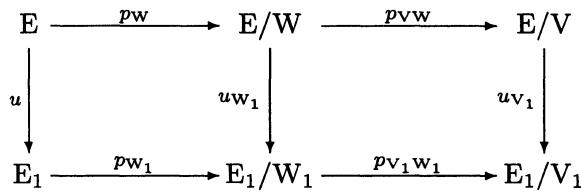
\includegraphics[keepaspectratio]{images/part002_2ec1bcbe.jpg}}

现在设 \(\mu = (\mu_{\mathrm{V}})_{\mathrm{V}\in \mathcal{F}(\mathrm{E})}\) 是 \(\mathbf{E}\) 上的前测度。对每个 \(\mathrm{V}_1\in \mathcal{F}(\mathrm{E}_1)\)，置

\[
\nu_ {\mathrm{V} _ {1}} = u _ {\mathrm{V} _ {1}} \left(\mu_ {u ^ {- 1} \left(\mathrm{V} _ {1}\right)}\right).\tag{1}
\]

前述图的交换性表明，族 \(\nu = (\nu_{\mathrm{V}_1})_{\mathrm{V}_1 \in \mathcal{F}(\mathrm{E}_1)}\) 是 \(\mathbf{E}_1\) 上的前测度。称 \(\nu\) 为 \(\mu\) 在 \(u\) 下的像，并记为 \(u(\mu)\)。

设 \(\lambda\) 是 E 上的有界测度，且 \(u(\lambda)\) 是 \(E_{1}\) 上的测度，是 \(\lambda\) 在 u 下的像。若前测度 \(\mu\) 与 \(\lambda\) 对应，则前测度 \(u(\mu)\) 与 \(u(\lambda)\) 对应。这由前述图的交换性得出。

设 \(V \in \mathcal{F}(E)\)。显然，定义在 \(E/V\) 上的、\(\mu\) 经典范映射 \(p_V: E \to E/V\) 得到的像前测度与测度 \(\mu_V\) 对应。

设 \(u_{1}\) 是从 \(E_{1}\) 到局部凸空间 \(E_{2}\) 的连续线性映射。容易证明关系

\[
(u _ {1} \circ u) (\mu) = u _ {1} (u (\mu))
\]

（前测度像的传递性）。

\subsection{前测度的傅里叶变换}

设 E 是局部凸空间，且 \(\mu = (\mu_{\mathrm{V}})_{\mathrm{V} \in \mathcal{F}(\mathrm{E})}\) 是 E 上的前测度。对 E 上的每个连续线性形式 \(x'\)，记 \(\mu_{x'}\) 为前测度 \(x'\) 经 \(\mu\) 作用后在 R 上得到的测度。称 \(\mu\) 的傅里叶变换为定义在 \(F\mu\) 上的函数 \(E'\)，由下式给出

\[
(\mathcal {F} \mu) (x ^ {\prime}) = \int_ {\mathbf {R}} e ^ {i t} d \mu_ {x ^ {\prime}} (t).\tag{2}
\]

设 \(\lambda\) 是 E 上的有界测度。称 \(\lambda\) 的傅里叶变换为定义在 \(\mathbf{E}'\) 上的函数，由下式给出

\[
(\mathcal {F} \lambda) (x ^ {\prime}) = \int_ {\mathrm{E}} e ^ {i \langle x, x ^ {\prime} \rangle} d \lambda (x).\tag{3}
\]

设 \(\mu\) 是与 \(\lambda\) 对应的前测度。对每个 \(x' \in E'\)，定义在 \(\mu_{x'}\) 上的测度 \(\mathbf{R}\) 是在映射 \(x': \mathrm{E} \to \mathbf{R}\) 下测度 \(\lambda\)（定义在 \(\mathrm{E}\) 上）的像；由公式 (2) 和 (3) 立即推出 \(\mathcal{F}\mu = \mathcal{F}\lambda\)。

设 \(\mu\) 是 \(\mathbf{E}\) 上的任意前测度，且 \(u\) 是从 \(\mathbf{E}\) 到局部凸空间 \(\mathbf{E}_1\) 的连续线性映射。记 \(^t u\) 为从 \(\mathbf{E}_1'\) 到 \(\mathbf{E}'\) 的线性映射，它是 \(u\) 的转置；并记 \(\nu\) 为前测度 \(u(\mu)\)，定义在 \(\mathbf{E}_1\) 上。对每个 \(x_1' \in \mathbf{E}_1'\)，有 \(^t u(x_1') = x_1' \circ u\)，从而

\[
\nu_ {x _ {1} ^ {\prime}} = x _ {1} ^ {\prime} (\nu) = x _ {1} ^ {\prime} (u (\mu)) = \left(x _ {1} ^ {\prime} \circ u\right) (\mu) = \mu^ {t} u \left(x _ {1} ^ {\prime}\right).
\]

因此，

\[
\mathscr {F} (u (\mu)) = (\mathscr {F} \mu) \circ {} ^ {t} u.\tag{4}
\]

特别地，对 \(p_{V}\) 取从 E 到 E/V 的典范映射 \(V \in \mathcal{F}(E)\)（\(p_{\mathrm{V}}(\mu)\)）。定义在 E/V 上的前测度 \(\mu_{V}\) 与测度 \(^{t}p_{V}\) 对应，而 \(V^{\circ}\) 将 E/V 的对偶同构地映到 E' 中与 V 正交的子空间 \(E'\)。若借助 \((\mathrm{E}/\mathrm{V})'\) 将 \(V^{\circ}\) 与 \(^{t}p_{V}\) 识别，则

\[
(\mathcal {F} \mu) (x ^ {\prime}) = \int_ {\mathrm{E} / \mathrm{V}} e ^ {i \langle x, x ^ {\prime} \rangle} d \mu_ {\mathrm{V}} (x)\tag{5}
\]

对 \(x' \in V^{\circ}\) 都有。\(E' = \bigcup_{V \in \mathcal{F}(E)} V^{\circ}\)，所以前述公式刻画了函数 \(\mathcal{F}\mu\) 在 \(E'\) 上。最后，在 (5) 中置 \(x' = 0\)，可见 \(\mu\) 的总质量等于 \((\mathcal{F}\mu)(0)\)。

命题 3. --- 设 E 是局部凸空间。映射 \(\mu \mapsto \mathcal{F}\mu\) 从 E 上的前测度集合到 E' 上的函数集合是单射。

公式 (5) 使问题归结为 E 有限维的情形；由于每个有限维空间都同构于某个 \(R^{n}\)，甚至不妨设存在整数 \(n \geqslant 0\)，使得 \(E = R^{n}\)。因此需要证明：若 \(\mu\) 是 \(R^{n}\) 上的有界测度（不一定为正），且

\[
\int_ {\mathbf {R} ^ {n}} e ^ {i \langle x, y \rangle} d \mu (x) = 0
\]

对每个线性形式 \(y\)（其定义域为 \(\mathbf{R}^n\)），上述等式都成立，则 \(\mu = 0\)。

对每个整数 \(m \geqslant 0\)，令 \(\mathbf{G}_m\) 为 \(m \cdot \mathbf{Z}^n\) 在 \(\mathbf{R}^n\) 中的子群。记 \(\mathcal{C}_m\) 为连续函数 \(f\) 所成的向量空间，其中 f 定义在 \(\mathbf{R}^n\) 上并满足 \(f(x + a) = f(x)\) 对 \(x \in \mathbf{R}^n\) 和 \(a \in \mathbf{G}_m\) 成立。由 GT, X, §4, No.~4 的命题 8，\(\mathcal{C}_m\) 中每个函数都是形如 \(x \mapsto e^{2\pi i\langle x,q\rangle}\)（其中 \(q \in m^{-1} \cdot \mathbf{Z}^n\)）的函数的有限线性组合的一致极限。因此，\(\mu(f) = 0\) 对每个函数 \(f \in \mathcal{C}_m\) 成立。

设 \(f\) 是 \(\mathbf{R}^n\) 上具有紧支集的连续函数。对每个整数 \(m \geqslant 0\)，置 \(f_m(x) = \sum_{q \in G_m} f(x + q)\)。显然，对每个 \(x \in \mathbf{R}^n\)，上述级数只有有限项，且 \(f_m\) 属于 \(\mathcal{C}_m\)。此外，容易看出序列 \((f_m)\) 在每个紧集上一致收敛到 \(f\)，并且存在常数 \(C \geqslant 0\)，使得 \(|f_m| \leqslant C\) 对所有 \(m\) 成立。因此，由 §5 第 6 号命题 12，\(\mu(f) = \lim_{m \to \infty} \mu(f_m)\)。由于 \(f_m \in \mathcal{C}_m\)，有 \(\mu(f_m) = 0\)，最终得到 \(\mu(f) = 0\)。故 \(\mu = 0\)。

*备注。 --- 当 E 有限维时，E 的每个特征都具有形式 \(x \mapsto e^{i\langle x,x' \rangle}\)，其中 \(x' \in \mathrm{E}'\)（Théor. spect., 第 II 章 §1, No.~9, 命题 12 的推论 3）。此时，命题 3 由傅里叶变换的唯一性定理得出（同上，§1, No.~6, 命题 6 的推论）。*

\subsection{高斯积分的计算}

引理 1. --- 对每个整数 \(n \geqslant 0\)，

\begin{enumerate}
\def\labelenumi{(\arabic{enumi})}
\setcounter{enumi}{5}
\tightlist
\item
\end{enumerate}

\[
\int_ {\mathbf {R}} | x | ^ {n} e ^ {- x ^ {2} / 2} d x = 2 ^ {\frac {n + 1}{2}} \Gamma \left(\frac {n + 1}{2}\right)\tag{7}
\]

\[
\int_ {\mathbf {R}} x ^ {2 n} e ^ {- x ^ {2} / 2} d x = (2 \pi) ^ {1 / 2} \frac {(2 n) !}{2 ^ {n} n !}\tag{8}
\]

\[
\int_ {\mathbf {R}} x ^ {2 n + 1} e ^ {- x ^ {2} / 2} d x = 0.
\]

回忆公式

\[
\Gamma (s) = \int_ {0} ^ {\infty} u ^ {s - 1} e ^ {- u} d u\tag{9}
\]

该公式对每个实数 \(s > 0\) 都成立（FRV, VII, §1, No.~3, 命题 3）。作变量代换 \(x = (2u)^{1/2}\)，由 (9) 得到

\[
\int_ {0} ^ {\infty} x ^ {n} e ^ {- x ^ {2} / 2} d x = \int_ {0} ^ {\infty} (2 u) ^ {n / 2} e ^ {- u} \frac {1}{2} 2 ^ {1 / 2} u ^ {- 1 / 2} d u = 2 ^ {\frac {n - 1}{2}} \Gamma \left(\frac {n + 1}{2}\right),
\]

从而得到公式 (6)，因为

\[
\int_ {\mathbf {R}} | x | ^ {n} e ^ {- x ^ {2} / 2} d x = 2 \int_ {0} ^ {\infty} x ^ {n} e ^ {- x ^ {2} / 2} d x.
\]

公式 (7) 由 (6) 及关系

\[
\Gamma \left(n + \frac {1}{2}\right) = \pi^ {1 / 2} \frac {(2 n) !}{2 ^ {2 n} n !}.\tag{10}
\]

当 \(n = 0\) 时，该关系化为 \(\Gamma(\frac{1}{2}) = \pi^{1/2}\)，即 FRV, VII, §1, No.~3 的公式 (21)。一般情形则对 \(n\) 作归纳，并利用关系 \(\Gamma(x + 1) = x \cdot \Gamma(x)\) 得到（同上，§1, No.~1）。

最后，公式 (8) 由函数 \(x \mapsto x^{2n+1}e^{-x^2/2}\) 为奇函数这一事实得出。

引理 2. --- 对每个复数 y，

\[
(2 \pi) ^ {- 1 / 2} \int_ {\mathbf {R}} e ^ {- x ^ {2} / 2} e ^ {i x y} d x = e ^ {- y ^ {2} / 2}.\tag{11}
\]

特别地，

\[
(2 \pi) ^ {- 1 / 2} \int_ {\mathbf {R}} e ^ {- x ^ {2} / 2} d x = 1.
\]

作变量代换 \(x \mapsto -x\)，得到

\[
(2 \pi) ^ {- 1 / 2} \int_ {\mathbf {R}} e ^ {- x ^ {2} / 2} e ^ {i x y} d x = (2 \pi) ^ {- 1 / 2} \int_ {\mathbf {R}} e ^ {- x ^ {2} / 2} e ^ {- i x y} d x;
\]

由于 \(\cos u = \frac{e^{iu} + e^{-iu}}{2}\) 对每个复数 \(u\) 成立，所以

\[
(2 \pi) ^ {- 1 / 2} \int_ {\mathbf {R}} e ^ {- x ^ {2} / 2} e ^ {i x y} d x = (2 \pi) ^ {- 1 / 2} \int_ {\mathbf {R}} e ^ {- x ^ {2} / 2} \cos x y d x.\tag{12}
\]

对每个整数 \(n \geqslant 0\)，置

\[
g _ {n} (x) = (- 1) ^ {n} (2 \pi) ^ {- 1 / 2} \frac {(x y) ^ {2 n}}{(2 n) !} e ^ {- x ^ {2} / 2}.
\]

由 (7)，

\begin{enumerate}
\def\labelenumi{(\arabic{enumi})}
\setcounter{enumi}{12}
\tightlist
\item
\end{enumerate}

\[
\int_ {\mathbf {R}} | g _ {n} (x) | d x = \frac {1}{n !} \biggl (\frac {| y | ^ {2}}{2} \biggr) ^ {n}\tag{14}
\]

\[
\int_ {\mathbf {R}} g _ {n} (x) d x = \frac {1}{n !} \Big (- \frac {y ^ {2}}{2} \Big) ^ {n},
\]

从而

\[
\sum_ {n = 0} ^ {\infty} \int_ {\mathbf {R}} | g _ {n} (x) | d x = e ^ {| y | ^ {2} / 2} <   + \infty .
\]

此外，

\[
(2 \pi) ^ {- 1 / 2} e ^ {- x ^ {2} / 2} \cos x y = \sum_ {n = 0} ^ {\infty} g _ {n} (x),
\]

这个等式可以逐项积分，从而得到

\[
(2 \pi) ^ {- 1 / 2} \int_ {\mathbf {R}} e ^ {- x ^ {2} / 2} \cos x y d x = \sum_ {n = 0} ^ {\infty} \int_ {\mathbf {R}} g _ {n} (x) d x = e ^ {- y ^ {2} / 2}
\]

根据 (14)，公式 (11) 随即由 (12) 得出。

\subsection{高斯前测度与测度}

命题 4. --- 设 E 是局部凸空间。对 \(E'\) 上的每个正二次型 Q，存在且仅存在一个 E 上的前测度 \(\Gamma_{Q}\)，使得 \(F\Gamma_{Q}=e^{-Q/2}\)。\(\Gamma_{Q}\) 的总质量等于 1。

\(\Gamma_{Q}\) 的唯一性由第 3 号命题 3 得出。\(\Gamma_{Q}\) 的总质量等于 \((\mathcal{F}\Gamma_{\mathrm{Q}})(0)=e^{-\mathrm{Q}(0)/2}=1\)。我们将分阶段证明存在性。

\begin{enumerate}
\def\labelenumi{\Alph{enumi})}
\tightlist
\item
  E 为 n 维，且 Q 非退化。
\end{enumerate}

由第 4 号引理 2，测度 \(\gamma_{1}\) 在 R 上具有密度 \(t \mapsto (2\pi)^{-1/2}e^{-t^{2}/2}\)，有界且总质量为 1。置 \(\gamma = \gamma_{1} \otimes \cdots \otimes \gamma_{1}\)（n 个因子）。由第 4 号引理 2，得到

\[
\begin{array}{r l} & {\int_ {\mathbf {R} ^ {n}} e ^ {i (a _ {1} t _ {1} + \dots + a _ {n} t _ {n})} d \gamma (t _ {1}, \ldots , t _ {n}) = \prod_ {j = 1} ^ {n} \int_ {\mathbf {R}} e ^ {i a _ {j} t} d \gamma_ {1} (t)} \\ & {\qquad = \prod_ {j = 1} ^ {n} (2 \pi) ^ {- 1 / 2} \int_ {\mathbf {R}} e ^ {i a _ {j} t} e ^ {- t ^ {2} / 2} d t} \\ & {\qquad = \prod_ {j = 1} ^ {n} e ^ {- a _ {j} ^ {2} / 2}} \\ & {\qquad = \exp \big (- \frac {1}{2} (a _ {1} ^ {2} + \dots + a _ {n} ^ {2}) \big).} \end{array}
\]

由于 Q 正且非退化，存在一个基 \((e_{1}^{\prime},\ldots,e_{n}^{\prime})\)，属于 \(E^{\prime}\)，且关于 Q 是正交规范的（Alg., 第 IX 章 §7, No.~1）。记从 E 到 \(x\mapsto(e_{1}^{\prime}(x),\ldots,e_{n}^{\prime}(x))\) 的同构 \(R^{n}\) 为 f，并以 \(\Gamma_{Q}\) 表示测度 \(f^{-1}(\gamma)\)（定义在 E 上）。设 \(x^{\prime}=a_{1}e_{1}^{\prime}+\cdots+a_{n}e_{n}^{\prime}\) 属于 \(E^{\prime}\)；则 \(x^{\prime}\big(f^{-1}(t_{1},\ldots,t_{n})\big)=\sum_{j=1}^{n}t_{j}a_{j}\) 对实数 \(t_{1},\ldots,t_{n}\) 成立，从而

\[
\begin{array}{l} \int_ {\mathbf {E}} e ^ {i \langle x, x ^ {\prime} \rangle} d \Gamma_ {\mathbf {Q}} (x) = \int_ {\mathbf {R} ^ {n}} e ^ {i (a _ {1} t _ {1} + \dots + a _ {n} t _ {n})} d \gamma (t _ {1}, \ldots , t _ {n}) \\ \qquad = \exp \big (- \frac {1}{2} (a _ {1} ^ {2} + \dots + a _ {n} ^ {2}) = \exp \big (- \frac {1}{2} \mathbf {Q} (x ^ {\prime}) \big). \end{array}
\]

因此，\(\mathcal{F}\Gamma_{\mathrm{Q}} = e^{-\mathrm{Q} / 2}\)。

\begin{enumerate}
\def\labelenumi{\Alph{enumi})}
\setcounter{enumi}{1}
\tightlist
\item
  E 有限维。
\end{enumerate}

令 N 为由 \(E'\) 中的 \(x'\)（满足 \(Q(x') = 0\)）所成的线性子空间。记 N 在 E 中的正交补为 M，记从 M 到 E 的典范嵌入为 j。线性映射 \({}^{t}j : E' \to M'\) 是满射，核为 N，因此在 \(M'\) 上存在非退化正二次型 q，使得 \(Q = q \circ {}^{t}j\)。由前面所述，在 M 上存在有界测度 \(\Gamma\)，使得 \(F\Gamma = e^{-q/2}\)。置 \(\Gamma_{Q} = j(\Gamma)\)，则有

\[
\mathcal {F} \Gamma_ {\mathrm{Q}} = (\mathcal {F} \Gamma) \circ {} ^ {t} j = \exp (- q \circ {} ^ {t} j / 2) = e ^ {- \mathrm{Q} / 2}
\]

由第 3 号的公式 (4)。
